\documentclass[11pt]{article}

%%%%%%%%%%%%%%%%%%%%%%%%%%%%%%%%%%%%%%%%%%%%%%%%%%%%%%%%%%%%
% Page layout and typography
%%%%%%%%%%%%%%%%%%%%%%%%%%%%%%%%%%%%%%%%%%%%%%%%%%%%%%%%%%%%
\usepackage[margin=1in]{geometry}
\usepackage[
  protrusion=true,
  activate={true,nocompatibility},
  final,
  tracking=true,
  kerning=true,
  factor=1100
]{microtype}
\SetTracking{encoding={*}, shape=sc}{40}

\usepackage{lmodern}
\usepackage[T1]{fontenc}

%%%%%%%%%%%%%%%%%%%%%%%%%%%%%%%%%%%%%%%%%%%%%%%%%%%%%%%%%%%%
% Math packages
%%%%%%%%%%%%%%%%%%%%%%%%%%%%%%%%%%%%%%%%%%%%%%%%%%%%%%%%%%%%
\usepackage{amsmath,amssymb,amsfonts,amsthm}
\usepackage{mathtools}

%%%%%%%%%%%%%%%%%%%%%%%%%%%%%%%%%%%%%%%%%%%%%%%%%%%%%%%%%%%%
% Figures, plots, algorithms, code
%%%%%%%%%%%%%%%%%%%%%%%%%%%%%%%%%%%%%%%%%%%%%%%%%%%%%%%%%%%%
\usepackage{graphicx}
\usepackage{tikz}
\usepackage{float}
\usepackage{pgfplots}
\pgfplotsset{compat=1.18}
\usetikzlibrary{shapes.geometric, arrows.meta, positioning, fit, shadows, patterns}

\usepackage{algorithm}
\usepackage[noend]{algpseudocode}

\usepackage{listings}
\usepackage{xcolor}
\usepackage{adjustbox}
\usepackage{placeins}
\usepackage{stfloats}
\usepackage{booktabs}
\usepackage{array}

%%%%%%%%%%%%%%%%%%%%%%%%%%%%%%%%%%%%%%%%%%%%%%%%%%%%%%%%%%%%
% Links and references
%%%%%%%%%%%%%%%%%%%%%%%%%%%%%%%%%%%%%%%%%%%%%%%%%%%%%%%%%%%%
\usepackage[hidelinks]{hyperref}
\usepackage[nameinlink,capitalise]{cleveref}

%%%%%%%%%%%%%%%%%%%%%%%%%%%%%%%%%%%%%%%%%%%%%%%%%%%%%%%%%%%%
% Code style
%%%%%%%%%%%%%%%%%%%%%%%%%%%%%%%%%%%%%%%%%%%%%%%%%%%%%%%%%%%%
\usepackage{inconsolata}

\lstdefinestyle{rgcode}{
  language=C,
  basicstyle=\scriptsize\ttfamily,
  numbers=left,
  numberstyle=\tiny,
  numbersep=6pt,
  xleftmargin=2em,
  frame=lines,
  rulecolor=\color{black},
  breaklines=true,
  breakindent=0pt,
  showstringspaces=false,
  captionpos=b
}

\lstset{
  basicstyle=\small\ttfamily,
  breaklines=true,
  frame=single,
  numbers=none,
  showstringspaces=false,
  morekeywords={uint32_t,uint64_t,int64_t,struct},
  keywordstyle=\color{blue},
  stringstyle=\color{red},
  commentstyle=\color{green!60!black},
  columns=flexible,
  keepspaces=true
}

%%%%%%%%%%%%%%%%%%%%%%%%%%%%%%%%%%%%%%%%%%%%%%%%%%%%%%%%%%%%
% Theorem environments
%%%%%%%%%%%%%%%%%%%%%%%%%%%%%%%%%%%%%%%%%%%%%%%%%%%%%%%%%%%%
\newtheorem{theorem}{Theorem}[section]
\newtheorem{lemma}[theorem]{Lemma}
\newtheorem{proposition}[theorem]{Proposition}
\newtheorem{claim}[theorem]{Claim}
\newtheorem{corollary}[theorem]{Corollary}

\theoremstyle{definition}
\newtheorem{definition}[theorem]{Definition}
\newtheorem{construction}[theorem]{Construction}
\newtheorem{remark}[theorem]{Remark}
\newtheorem{assumption}[theorem]{Assumption}

%%%%%%%%%%%%%%%%%%%%%%%%%%%%%%%%%%%%%%%%%%%%%%%%%%%%%%%%%%%%
% Macros
%%%%%%%%%%%%%%%%%%%%%%%%%%%%%%%%%%%%%%%%%%%%%%%%%%%%%%%%%%%%
\newcommand{\F}{\mathbb{F}}
\newcommand{\Z}{\mathbb{Z}}

\newcommand{\WHIR}{\mathsf{WHIR}}
\newcommand{\CP}{\mathsf{CP}}
\newcommand{\SNARK}{\mathsf{SNARK}}
\newcommand{\Acc}{\mathsf{Acc}}
\newcommand{\Fold}{\mathsf{Fold}}
\newcommand{\Verify}{\mathsf{Verify}}
\newcommand{\Prove}{\mathsf{Prove}}
\newcommand{\Commit}{\mathsf{Commit}}
\newcommand{\Open}{\mathsf{Open}}

\newcommand{\Rwhir}{\mathcal{R}_{\mathsf{WHIRVerify}}}
\newcommand{\Rfold}{\mathcal{R}_{\mathsf{Fold}}}
\newcommand{\Rcp}{\mathcal{R}_{\mathsf{CPFold}}}
\newcommand{\Rbackend}{\mathcal{R}_{\mathsf{backend}}}
\newcommand{\Renc}{\mathcal{R}_{\mathsf{enc}}}

%%%%%%%%%%%%%%%%%%%%%%%%%%%%%%%%%%%%%%%%%%%%%%%%%%%%%%%%%%%%
% Title
%%%%%%%%%%%%%%%%%%%%%%%%%%%%%%%%%%%%%%%%%%%%%%%%%%%%%%%%%%%%
\title{\Large \bf WHIR Accumulation Through Lattice-Based Folding}

\author{
Paul Louis Robert Quesnot\\
EPFL
}

\date{\today}

%%%%%%%%%%%%%%%%%%%%%%%%%%%%%%%%%%%%%%%%%%%%%%%%%%%%%%%%%%%%
\begin{document}
%%%%%%%%%%%%%%%%%%%%%%%%%%%%%%%%%%%%%%%%%%%%%%%%%%%%%%%%%%%%

\maketitle

\begin{abstract}
Accumulation is a natural way to avoid verifying many succinct proofs independently, but
applying it to hash-based proof systems requires accumulating verifier claims rather than
proof byte strings. We study this question for WHIR, a fast Reed--Solomon
proximity-testing based backend, and Symphony-style lattice-based folding.

Our construction models typed accumulation inputs as WHIR proof-validity claims,
folds these claims through a lattice-based accumulator, and certifies the folding
transition with a commit-and-prove relation whose backend is again WHIR.

The implementation shows that the public-verifier boundary can be preserved in explicit
accumulation routes, while identifying the typed CP relation, transcript binding, and relation
encoding as the main bottlenecks toward a production-authoritative accumulator.
 \end{abstract}

\vspace{1em}

\noindent\textbf{Keywords.}
WHIR, accumulation, folding schemes, lattice-based commitments, commit-and-prove SNARKs,
interactive oracle proofs, proof systems.

\newpage

\tableofcontents

\newpage

%%%%%%%%%%%%%%%%%%%%%%%%%%%%%%%%%%%%%%%%%%%%%%%%%%%%%%%%%%%%
\section{Introduction}
\label{sec:introduction}
%%%%%%%%%%%%%%%%%%%%%%%%%%%%%%%%%%%%%%%%%%%%%%%%%%%%%%%%%%%%

\subsection{Motivation}
\label{sec:motivation}
WHIR is already compelling as a proof backend in its own right. It offers a fast
hash-based polynomial-commitment architecture, succinct proofs built from
Merkle-committed polynomial evaluations, and a public verifier boundary that fits
naturally with modern hash-based proof infrastructure. In the current repository,
this is not just a design goal: WHIR-backed public verification already exists as
an authoritative public-only route. WHIR provides a fast interactive-oracle style
polynomial-commitment backend based on Reed--Solomon proximity-testing ideas,
and Symphony provides the high-arity lattice-based folding and commit-and-prove
setting in which we study accumulation~\cite{WHIR,Symphony}.

Even so, verifying many WHIR proofs independently still repeats verifier work.
Each proof must be checked against its public inputs, its transcript commitments,
its derived challenges, and its folded-output boundary. If an application needs to
validate many such proofs, then the backend may already be succinct, but the
verifier still performs the same pattern of checks over and over again.

This is exactly the setting in which folding suggests accumulation. Rather than
checking many WHIR-backed claims independently, one would like to combine them
into a single accumulator transition and certify that transition succinctly. If
successful, this preserves the benefits of WHIR as a standalone backend while also
amortizing repeated verifier work across many claims.

The subtlety is that the object to be accumulated is not the proof bytes themselves.
For WHIR-like systems, what matters is the proof-validity claim induced by each
proof: public inputs, Fiat--Shamir commitments, transcript
roots/digests, derived challenges, opened evaluations, and folded-output
semantics must remain bound to the same verification relation. A sound
accumulation scheme must therefore fold verification claims, not raw proof
payloads.

\subsection{Problem Statement}
\label{sec:problem-statement}

The mathematical goal of this report is to describe an accumulation procedure for
WHIR-backed proof-validity claims. Given an old accumulator
$\Acc_{\mathsf{old}}$ and a batch of WHIR-backed claims, the prover should produce
a new accumulator $\Acc_{\mathsf{new}}$ together with an accumulation proof
$\Pi_{\mathsf{acc}}$ such that acceptance implies that the declared accumulator
transition is valid and that the accumulated WHIR verification claims hold,
except with the explicit error inherited from the underlying backend, folding,
and binding assumptions.

To make that goal meaningful, the public-verifier boundary must remain intact.
Verification should be public-only and fail-closed. Public inputs, relation
metadata, Fiat--Shamir commitments and their roots, challenge derivation,
challenge-to-$\beta$ binding, folded-output algebra, original Ajtai opening
validity, original R1CS validity, and accumulator-transition consistency must all
be tied to the same proof object. If any of those checks escape into witness-side
replay, debug-only helpers, or silent fallback routes, then the resulting object
is not a genuine public accumulator.

Within the current implementation, this problem appears through three distinct
routes. First, the default public API
\texttt{verify\_public}/\texttt{verify\_v2} provides the authoritative WHIR+WHIR
public verifier and serves as the baseline public boundary. Second, the explicit
opt-in \emph{single-oracle} accumulation route is the current full accumulator
workload path and is \emph{NonZK integrity-only}. Third, the repository
implements an explicit \emph{multi-oracle} accumulation route for same-shape,
nonempty NonZK transitions.
These route names are implementation labels; the conceptual distinction is
between baseline public verification, explicit full-workload accumulation, and
integrated one-proof accumulation. The single-oracle versus multi-oracle
technical distinction is developed in Section~\ref{sec:single-vs-multi-oracle}.
The rest of the report studies accumulation against this three-route background.
%%%%%%%%%%%%%%%%%%%%%%%%%%%%%%%%%%%%%%%%%%%%%%%%%%%%%%%%%%%%
\subsection{Contributions}
\label{sec:contributions}
%%%%%%%%%%%%%%%%%%%%%%%%%%%%%%%%%%%%%%%%%%%%%%%%%%%%%%%%%%%%
The main contributions of this report are the following.

\begin{itemize}
  \item \textbf{Formalization.} We isolate the right accumulation object for the
  WHIR setting: proof-validity claims with an explicit public boundary and
  transcript-binding requirements.

  \item \textbf{Construction.} We describe a WHIR-backed accumulation
  architecture in which WHIR proof-validity claims are folded through a
  Symphony-style lattice accumulator and the resulting transition is certified by
  a CP relation proved with WHIR. We then map this construction to the
  implemented single-oracle and multi-oracle routes.

  \item \textbf{Completeness and soundness reduction.} We prove completeness
  of the abstract accumulator and reduce one-step public soundness to backend
  soundness, commitment binding, transcript binding, and row-level faithfulness
  of the typed implementation.

  \item \textbf{Implementation.} We map the construction to the current Symphony
  + WHIR codebase, emphasizing the public-proof boundary, the route split, and
  the concrete WHIR backend integration.

  \item \textbf{Evaluation.} We organize the performance story around the
  authoritative monolithic baseline, the explicit single-oracle accumulation
  route, and the integrated multi-oracle alternative.

  \item \textbf{Limitations.} We explain the current engineering boundary: the
  default public verifier is authoritative but still dominated by a large typed
  CP relation, and the next performance direction lies in more compressed
  SYMBT3/native multi-oracle structures.
\end{itemize}

%%%%%%%%%%%%%%%%%%%%%%%%%%%%%%%%%%%%%%%%%%%%%%%%%%%%%%%%%%%%
\section{Technical Overview}
\label{sec:technical-overview}
%%%%%%%%%%%%%%%%%%%%%%%%%%%%%%%%%%%%%%%%%%%%%%%%%%%%%%%%%%%%
%%%%%%%%%%%%%%%%%%%%%%%%%%%%%%%%%%%%%%%%%%%%%%%%%%%%%%%%%%%%
\subsection{High-Level Architecture}
\label{sec:high-level-architecture}
%%%%%%%%%%%%%%%%%%%%%%%%%%%%%%%%%%%%%%%%%%%%%%%%%%%%%%%%%%%%
At a high level, the repository implements a common stack and then exposes
multiple public routes through that stack. The underlying mathematical objects
are source R1CS/GR1CS-style claims together with Ajtai commitment openings. An
individual WHIR proof certifies such a source claim. For accumulation, however,
the system first views each statement/proof pair as a public WHIR proof-validity
claim. Symphony's high-arity folding machinery is applied to those claims, the
resulting folding step is certified by a commit-and-prove relation, and that CP
relation is proved together with the folded-output boundary consumed by the
verifier.

A useful stack-level picture is shown in \Cref{fig:high-level-architecture}.

\begin{figure}[H]
\centering
\begin{adjustbox}{max width=\linewidth}
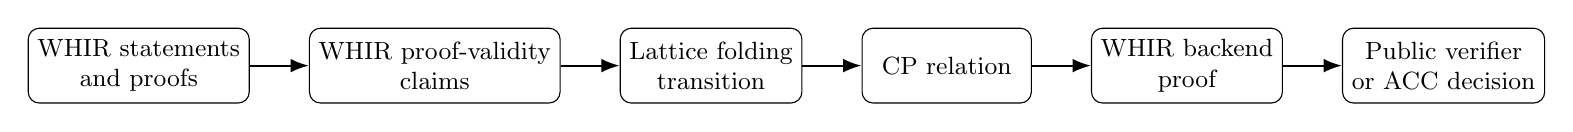
\begin{tikzpicture}[
  node distance=0.75cm,
  font=\small,
  box/.style={draw, rounded corners, align=center, minimum width=2.15cm, minimum height=0.95cm},
  arrow/.style={-Latex, thick}
]
\node[box] (whir) {WHIR statements\\and proofs};
\node[box, right=of whir] (claims) {WHIR proof-validity\\claims};
\node[box, right=of claims] (fold) {Lattice folding\\transition};
\node[box, right=of fold] (cp) {CP relation};
\node[box, right=of cp] (backend) {WHIR backend\\proof};
\node[box, right=of backend] (verify) {Public verifier\\or ACC decision};

\draw[arrow] (whir) -- (claims);
\draw[arrow] (claims) -- (fold);
\draw[arrow] (fold) -- (cp);
\draw[arrow] (cp) -- (backend);
\draw[arrow] (backend) -- (verify);
\end{tikzpicture}
\end{adjustbox}
\caption{High-level architecture of WHIR accumulation through lattice-based folding.}
\label{fig:high-level-architecture}
\end{figure}

In the current implementation, WHIR is the main backend for this stack. It
provides typed CP proofs and typed folded-output proofs over
\texttt{Poseidon2BabyBear} public digests, while preserving a public-only
verifier boundary for the authoritative public route.

%%%%%%%%%%%%%%%%%%%%%%%%%%%%%%%%%%%%%%%%%%%%%%%%%%%%%%%%%%%%
\subsection{What is Being Accumulated?}
\label{sec:what-is-being-accumulated}
%%%%%%%%%%%%%%%%%%%%%%%%%%%%%%%%%%%%%%%%%%%%%%%%%%%%%%%%%%%%
What is accumulated is not a vector of WHIR proof bytes. The accumulated object
is a family of \emph{WHIR proof-validity claims}. Each such claim includes the
public inputs, the relation metadata, the public Fiat--Shamir commitments, the
public roots and digests, the challenge binding, the commitment-opening algebra,
and the folded-output semantics that the verifier must ultimately trust.

Thus, throughout the report, a claim means the public WHIR verifier obligation
itself, not just a serialized proof object. Folding is sound only to the extent
that it preserves that obligation and its public bindings.

%%%%%%%%%%%%%%%%%%%%%%%%%%%%%%%%%%%%%%%%%%%%%%%%%%%%%%%%%%%%
\subsection{Public-Verifier Boundary}
\label{sec:public-verifier-boundary}
%%%%%%%%%%%%%%%%%%%%%%%%%%%%%%%%%%%%%%%%%%%%%%%%%%%%%%%%%%%%
\begin{definition}[Authoritative public verifier]
A verifier route is authoritative if its decision depends only on public inputs,
public proof objects, public transcript commitments, public digests, and public
backend proofs. It must not read witnesses, prover messages, Fiat--Shamir
openings, fold inputs, folded witnesses, or debug-only replay material.
Moreover, it must fail closed if the required typed backend verification is not
available.
\end{definition}

The authoritative public verifier is the default version-2 public proof route:
\texttt{ProofBundleV2}\slash\texttt{PublicProofBundle} and
\texttt{SymphonyProofV2}\slash\texttt{PublicSymphonyProof}, exposed through
\texttt{prove\_public} and \texttt{verify\_public} with
\texttt{prove\_v2}\slash\texttt{verify\_v2} as compatibility aliases. For WHIR+WHIR,
this route is authoritative: the CP backend proves the typed CP relation, the
output backend proves transcript binding for the folded output, the public digest
scheme is \texttt{Poseidon2BabyBear}, and verification succeeds using public data
only.

Concretely, the public verifier consumes caller-supplied public inputs and
relation metadata, public Fiat--Shamir commitments, the public roots and digests
\texttt{fs\_root}, \texttt{fold\_root}, \texttt{challenge\_digest}, and
\texttt{transcript\_seed\_digest}, the public folded-output instance, and the
WHIR CP/output proofs. It must not consume Fiat--Shamir openings, Fiat--Shamir
messages, fold inputs, original witnesses, folded witnesses, folding-proof
internals, or CP witness bundles. Public verification is also fail-closed: if
backend authority or typed verification is missing, the route rejects rather
than silently falling back to witness-side checks.

This monolithic WHIR public verifier is therefore the correct baseline
implementation for the report. It is the first unoptimized implementation stage
in this codebase that establishes a real public-only boundary; every
accumulation route studied later must preserve the same semantic commitments at
that boundary.

%%%%%%%%%%%%%%%%%%%%%%%%%%%%%%%%%%%%%%%%%%%%%%%%%%%%%%%%%%%%
\subsection{Implementation Routes}
\label{sec:implementation-routes}
%%%%%%%%%%%%%%%%%%%%%%%%%%%%%%%%%%%%%%%%%%%%%%%%%%%%%%%%%%%%
The implementation routes relevant to this report are summarized in
\Cref{tab:route-taxonomy}. They should be read as three implementation-level
realizations of the same overall topic, each with a different role in the
report:
\begin{itemize}
  \item the authoritative public verifier provides the baseline public boundary;
  \item the single-oracle route provides the current explicit full-workload
  accumulation route;
  \item the multi-oracle route provides the integrated one-proof accumulation
  alternative.
\end{itemize}
This is a taxonomy, not a logical implication chain. The single-oracle and
multi-oracle routes are explicit routes that are compared against the baseline
public verifier; neither is a corollary of, nor a silent replacement for, the
default public route.

\begin{table}[H]
\centering
\small
\setlength{\tabcolsep}{3pt}
\renewcommand{\arraystretch}{1.15}
\begin{tabular}{>{\raggedright\arraybackslash}p{0.24\linewidth} >{\raggedright\arraybackslash}p{0.42\linewidth} >{\centering\arraybackslash}p{0.10\linewidth} >{\raggedright\arraybackslash}p{0.18\linewidth}}
\toprule
Route & Conceptual role & Default? & Status \\
\midrule
Product public verifier &
Baseline public-only WHIR+WHIR verification boundary &
Yes &
Correct monolithic baseline \\
Single-oracle (repo \texttt{K6a}) &
Explicit full-workload NonZK accumulation route &
No &
Implemented \\
Multi-oracle (repo \texttt{N8}) &
Integrated same-shape NonZK accumulation route using one WHIR proof &
No &
Implemented, opt-in, not production-reviewed \\
\bottomrule
\end{tabular}
\caption{Verification and accumulation routes used in this report.}
\label{tab:route-taxonomy}
\end{table}

The authoritative default exposes \texttt{prove\_public} and
\texttt{verify\_public}; \texttt{prove\_v2}\slash\texttt{verify\_v2} are
compatibility aliases. The
single-oracle route and the multi-oracle route are both explicit opt-in
accumulation routes. The single-oracle route is the current main full-workload
accumulation route; the multi-oracle route is the implemented integrated
alternative with explicit \texttt{ACC.P}\slash\texttt{ACC.V}\slash\texttt{ACC.D}
entry points. Their technical distinction is developed in Section~\ref{sec:single-vs-multi-oracle}.
Neither silently replaces the default public verifier.

%%%%%%%%%%%%%%%%%%%%%%%%%%%%%%%%%%%%%%%%%%%%%%%%%%%%%%%%%%%%
\subsection{Performance Direction}
\label{sec:performance-direction}
%%%%%%%%%%%%%%%%%%%%%%%%%%%%%%%%%%%%%%%%%%%%%%%%%%%%%%%%%%%%
The reason the story does not end at \texttt{verify\_public} is performance. The
default WHIR public verifier is authoritative and public-only, but it is still
built around a monolithic typed CP relation whose row count grows materially with
the folded workload. In other words, the baseline verifier is correct as a first
unoptimized, monolithic implementation of the public boundary, but it is not yet
the final cost profile one would want from an accumulated public route.

This motivates the broader SYMBT3/native multi-oracle direction. The report does
not need to center every intermediate experiment in that line, but it does need
to explain the performance motivation shared by the three routes above. The
baseline public verifier establishes the current authoritative boundary; the
single-oracle route is the current explicit accumulation realization studied
against that baseline; and the multi-oracle route is the integrated one-WHIR
alternative that explores a more compressed proof shape. The broader
native/multi-oracle work should therefore be read mainly as the performance
program that supports this line of refinement.

%%%%%%%%%%%%%%%%%%%%%%%%%%%%%%%%%%%%%%%%%%%%%%%%%%%%%%%%%%%%
\section{Preliminaries}
\label{sec:preliminaries}
%%%%%%%%%%%%%%%%%%%%%%%%%%%%%%%%%%%%%%%%%%%%%%%%%%%%%%%%%%%%

We recall only the notation, interfaces, and soundness properties used later.
The report treats WHIR, folding, commit-and-prove, and commitments as components
with specified public behavior; their internal constructions are not reproved.

\paragraph{Notation.}
For \(n\in\mathbb{N}\), write \([n]=\{1,\ldots,n\}\). The security parameter is
\(\lambda\), and \(\varepsilon(\lambda)\) denotes a negligible or explicitly
bounded failure probability. Public inputs appear before a semicolon and private
witness material after it:
\[
  R(x;w)=1.
\]
When no witness is shown, all inputs are public. We use
\(\mathsf{Digest}(\cdot)\) for a collision-resistant or random-oracle-derived
binding value, and \(H_{\mathsf{dom}}\) for a domain-separated random-oracle
call.

%%%%%%%%%%%%%%%%%%%%%%%%%%%%%%%%%%%%%%%%%%%%%%%%%%%%%%%%%%%%
\subsection{Interactive Oracle Proofs and SNARKs}
\label{sec:prelim-iops-snarks}
%%%%%%%%%%%%%%%%%%%%%%%%%%%%%%%%%%%%%%%%%%%%%%%%%%%%%%%%%%%%

An indexed relation is a family
\[
  R =
  \{R_{\mathsf{idx}}\}_{\mathsf{idx}},
\]
where \(\mathsf{idx}\) is a public index, \(x\) is a public instance, and \(w\)
is a witness. We write
\[
  R_{\mathsf{idx}}(x;w)=1
\]
when \(w\) is valid for \(x\). Here, indices include proof-system parameters,
relation identifiers, route metadata, and backend parameters.

A succinct argument system for \(R\) consists of a prover and verifier,
\[
  \Pi.\Prove(\mathsf{idx},x,w)\to \pi,
  \qquad
  \Pi.\Verify(\mathsf{idx},x,\pi)\to \{0,1\}.
\]
Completeness means honest proofs verify. The knowledge-style soundness form
used later says that an accepting proof implies, except with the stated error,
the existence of a witness satisfying the indexed relation.

We use IOP/SNARK terminology only at this interface level. Oracle messages,
Fiat--Shamir challenges, and openings matter in the report only insofar as they
are committed public data that the verifier statement binds.

%%%%%%%%%%%%%%%%%%%%%%%%%%%%%%%%%%%%%%%%%%%%%%%%%%%%%%%%%%%%
\subsection{WHIR}
\label{sec:prelim-whir}
%%%%%%%%%%%%%%%%%%%%%%%%%%%%%%%%%%%%%%%%%%%%%%%%%%%%%%%%%%%%

WHIR~\cite{WHIR} is used as a transparent, hash-based backend for encoded
relations:
\[
  \WHIR.\Prove(\mathsf{stmt},w)\to \Pi,
  \qquad
  \WHIR.\Verify(\mathsf{stmt},\Pi)\to \{0,1\}.
\]
The public statement \(\mathsf{stmt}\) contains the WHIR parameters, relation
identifier, public inputs, public transcript material, and any folded-output
boundary that the verifier is asked to trust.

We associate to WHIR a public verification relation
\[
  \Rwhir(\mathsf{stmt},\pi)=1,
\]
which holds exactly when the WHIR verifier accepts proof object \(\pi\) for
\(\mathsf{stmt}\). The report uses WHIR in two roles:
\begin{enumerate}
  \item input WHIR proofs \(\pi_i\), which define the WHIR proof-validity claims
        being accumulated;
  \item backend WHIR proofs \(\Pi_{\mathsf{cp}}\), which prove the encoded
        commit-and-prove relation certifying the folding transition.
\end{enumerate}
Soundness is used as a black-box implication: if
\[
  \WHIR.\Verify(\mathsf{stmt},\Pi)=1,
\]
then, except with the WHIR soundness error, the relation encoded by
\(\mathsf{stmt}\) is satisfiable.

%%%%%%%%%%%%%%%%%%%%%%%%%%%%%%%%%%%%%%%%%%%%%%%%%%%%%%%%%%%%
\subsection{Accumulation and Folding}
\label{sec:prelim-accumulation-folding}
%%%%%%%%%%%%%%%%%%%%%%%%%%%%%%%%%%%%%%%%%%%%%%%%%%%%%%%%%%%%

An accumulation scheme maintains a short public accumulator state. One step
absorbs a batch of claims into a new state and proves that the update is valid.
For WHIR proof-validity claims, the semantic folding transition is written
\[
  \Rfold\!\left(
    \Acc_{\mathsf{old}},
    \{\mathsf{Claim}_i\}_{i=1}^k,
    \Acc_{\mathsf{new}};
    w_{\mathsf{fold}}
  \right)=1.
\]
The witness \(w_{\mathsf{fold}}\) contains prover-side folding and opening
material. The public verifier does not read it directly; it verifies a proof of
the corresponding relation.

The relation enforces the supported claim shape, the prescribed linear or
lattice-based combination of old state and claim data, and preservation of the
public boundary: inputs, relation identifiers, transcript roots, challenge
digests, and folded-output data all remain bound to the same transition. The
Symphony-style layer is used only through this high-arity folding interface.

%%%%%%%%%%%%%%%%%%%%%%%%%%%%%%%%%%%%%%%%%%%%%%%%%%%%%%%%%%%%
\subsection{Commit-and-Prove SNARKs}
\label{sec:prelim-cp-snarks}
%%%%%%%%%%%%%%%%%%%%%%%%%%%%%%%%%%%%%%%%%%%%%%%%%%%%%%%%%%%%

A commit-and-prove relation checks ordinary algebraic constraints together with
consistency against committed data. Here it bridges the semantic folding
relation and the WHIR backend.

The public CP instance is written
\[
  I_{\mathsf{cp}}
  =
  \left(
    \Acc_{\mathsf{old}},
    \{\mathsf{Claim}_i\}_{i=1}^k,
    \Acc_{\mathsf{new}},
    \mathsf{params},
    \mathsf{tr}_{\mathsf{pub}}
  \right),
\]
where \(\mathsf{tr}_{\mathsf{pub}}\) contains public transcript-binding
material: relation identifiers, roots, digests, challenge digests, backend
parameters, and folded-output boundary data. The witness is
\[
  w_{\mathsf{cp}}
  =
  \left(
    w_{\mathsf{fold}},
    \mathsf{openings},
    \mathsf{aux}
  \right).
\]
The CP relation is denoted
\[
  \Rcp(I_{\mathsf{cp}};w_{\mathsf{cp}})=1.
\]

The role of \(\Rcp\) is to certify the folding transition without exposing
folding witnesses or openings. It must not weaken the folding statement: whenever
\[
  \Rcp(I_{\mathsf{cp}};w_{\mathsf{cp}})=1,
\]
the underlying folding relation must hold for the same public claims, the same
transcript-binding material, and the same folded-output boundary.

In the implementation, this CP relation is encoded as a WHIR backend statement
and proved using WHIR; there is no separate CP proof followed by a WHIR proof.

%%%%%%%%%%%%%%%%%%%%%%%%%%%%%%%%%%%%%%%%%%%%%%%%%%%%%%%%%%%%
\subsection{Lattice Commitments}
\label{sec:prelim-lattice-commitments}
%%%%%%%%%%%%%%%%%%%%%%%%%%%%%%%%%%%%%%%%%%%%%%%%%%%%%%%%%%%%

The folding layer uses lattice/Ajtai-style commitments to bind folding data and
witness material. We use only the interface
\[
  c \leftarrow \Commit(m;r),
\]
where \(m\) is the committed message and \(r\) is opening randomness or opening
material.

The property used later is binding: except with error
\(\varepsilon_{\mathsf{bind}}\), a commitment cannot be opened to two
inconsistent messages. Binding ties folding witnesses, claim encodings,
accumulator state, and CP witness material to the same committed data.

There are several commitment layers in the construction. Lattice commitments
bind folding data. The commit-and-prove layer binds witness material to the
public CP instance. WHIR uses hash/Merkle-style oracle commitments internally
when proving the encoded backend relation. These layers serve different roles
and must be tied to the same public statement by explicit transcript and digest
binding.

%%%%%%%%%%%%%%%%%%%%%%%%%%%%%%%%%%%%%%%%%%%%%%%%%%%%%%%%%%%%
\section{WHIR Accumulation Through Lattice-Based Folding}
\label{sec:whir-accumulation-through-lattice-based-folding}
%%%%%%%%%%%%%%%%%%%%%%%%%%%%%%%%%%%%%%%%%%%%%%%%%%%%%%%%%%%%

\subsection{Interface}
\label{sec:interface}

\begin{algorithm}[H]
\caption{\textsc{AccumulateWHIR}}
\begin{algorithmic}[1]
\Require Old accumulator $\Acc_{\mathsf{old}}$
\Require Public WHIR proof-validity inputs represented by an accumulation batch
\Ensure New accumulator $\Acc_{\mathsf{new}}$ and accumulation proof $\Pi_{\mathsf{acc}}$
\State Convert the batch inputs into WHIR proof-validity claims.
\State Fold the resulting claims using the lattice-based folding layer.
\State Form the CP instance $I_{\mathsf{cp}}$ and witness $w_{\mathsf{cp}}$ certifying the folding transition.
\State Encode $\Rcp(I_{\mathsf{cp}};w_{\mathsf{cp}})=1$ as a WHIR backend statement $\mathsf{stmt}_{\mathsf{cp}}$.
\State Produce $\Pi_{\mathsf{cp}} \leftarrow \WHIR.\Prove(\mathsf{stmt}_{\mathsf{cp}}, w_{\mathsf{cp}})$.
\State \Return $(\Acc_{\mathsf{new}}, \Pi_{\mathsf{acc}})$, where $\Pi_{\mathsf{acc}}$ contains $\Pi_{\mathsf{cp}}$ and the public CP instance.
\end{algorithmic}
\end{algorithm}

\subsection{From WHIR Proofs to Verification Claims}
\label{sec:whir-proof-validity-claims}

We now fix notation for the claim object introduced above. A WHIR prover
produces a proof object $\pi_i$ for a public verifier statement
$\mathsf{stmt}_i$; accumulation uses the corresponding verifier predicate:
\[
  (\mathsf{stmt}_i,\pi_i)
  \rightsquigarrow
  \Rwhir(\mathsf{stmt}_i,\pi_i)=1.
\]

\begin{definition}[WHIR proof-validity claim]
A WHIR proof-validity claim is a pair $(\mathsf{stmt},\pi)$ together with the
assertion
\[
  \Rwhir(\mathsf{stmt},\pi)=1,
\]
where $\mathsf{stmt}$ is the full public WHIR verifier statement and $\pi$ is the
corresponding WHIR proof object.
\end{definition}

The statement $\mathsf{stmt}_i$ is the full public statement at the WHIR verifier
boundary, not merely the original source relation. In particular, it contains the
declared WHIR parameters, relation metadata, public inputs, public transcript
commitments, roots and digests, challenge-binding data, and the folded-output
boundary that the verifier is asked to trust.

The accumulator therefore acts on \(\Rwhir(\mathsf{stmt}_i,\pi_i)=1\) together
with these public bindings. Later soundness statements rely on the folded claim
remaining the same verifier obligation as the ordinary WHIR relation
\(\Rwhir\).

Equivalently, for a batch of WHIR statements and proofs we write
\[
  \mathsf{Claim}_i :=
  (\mathsf{stmt}_i,\pi_i)
  \quad\text{with predicate}\quad
  \Rwhir(\mathsf{stmt}_i,\pi_i)=1,
  \qquad i\in[k].
\]
The accumulation procedure acts on the family
$\{\mathsf{Claim}_i\}_{i=1}^k$. Later sections specify how these claims are
folded, how the folding transition is certified by a commit-and-prove relation,
and how that relation is encoded into the WHIR backend. The soundness of the
overall construction depends on this encoding proving the same public relation.

\subsection{Lattice-Based Folding of Claims}
\label{sec:lattice-folding-of-claims}

After converting WHIR statement/proof pairs into proof-validity claims, the
accumulator must combine a batch of such claims into one transition.
Let $\mathsf{Claim}_1,\ldots,\mathsf{Claim}_k$ be the WHIR proof-validity
claims defined in Section~\ref{sec:whir-proof-validity-claims}.
The role of the folding layer is to absorb the family
$\{\mathsf{Claim}_i\}_{i=1}^k$ into a transition from an old accumulator
$\Acc_{\mathsf{old}}$ to a new accumulator $\Acc_{\mathsf{new}}$.

At this level, the folding layer should be understood as an accumulator update
relation. It does not merely hash together the input proof objects, nor does it
verify each WHIR proof independently. Instead, it constructs a folded public
instance whose validity is intended to imply that the input proof-validity claims
have been correctly incorporated into the accumulator state.

We write the abstract folding relation as
\[
  \Rfold\!\left(
    \Acc_{\mathsf{old}},
    \{\mathsf{Claim}_i\}_{i=1}^k,
    \Acc_{\mathsf{new}};
    w_{\mathsf{fold}}
  \right)=1,
\]
where $w_{\mathsf{fold}}$ denotes the private material needed to witness the
folding transition. In the implementation this material may include commitment
openings, folding witnesses, and other prover-side data needed to justify the
new folded state. The public verifier will not read this material directly; it
will only check a proof that the corresponding relation is satisfied.

At this point $\Rfold$ is an abstract relation: it specifies the semantic
accumulator transition, not yet the concrete arithmetized relation proved by
WHIR.

The folding transition is required to bind the following public data:
\begin{enumerate}
  \item the old accumulator $\Acc_{\mathsf{old}}$;
  \item the full batch of WHIR proof-validity claims
        $\{\mathsf{Claim}_i\}_{i=1}^k$;
  \item the declared relation and backend parameters;
  \item the Fiat--Shamir transcript material used to derive the folding
        challenges;
  \item the folded-output boundary that becomes part of
        $\Acc_{\mathsf{new}}$.
\end{enumerate}

Concretely, the folding challenge vector should be derived from public binding
material, rather than chosen independently by the prover. Schematically, one may
view it as
\[
  \boldsymbol{\beta}
  :=
  H_{\mathsf{fold}}\!\left(
    \Acc_{\mathsf{old}},
    \mathsf{Digest}(\mathsf{Claim}_1,\ldots,\mathsf{Claim}_k),
    \mathsf{params}
  \right),
\]
where $H_{\mathsf{fold}}$ denotes the domain-separated random-oracle call used
for folding. The exact transcript format is implementation-dependent, but the
soundness requirement is not: the same public material that determines the
claims must also determine the folding challenges.

The relation $\Rfold$ enforces three kinds of consistency.

First, it enforces \emph{shape consistency}: the claims being folded must belong
to the same supported accumulation shape. In the implemented NonZK routes this
means, in particular, that the accumulation batch is nonempty and that the claims
have compatible relation and backend metadata.

Second, it enforces \emph{algebraic folding consistency}: the new folded state
must be the prescribed linear or lattice-based combination of the previous state
and the input claim data under the challenge vector $\boldsymbol{\beta}$. This
is the part of the construction inherited from the Symphony-style folding layer.

Third, it enforces \emph{public-boundary consistency}: the accumulator update
must preserve the same public statement data that the verifier is asked to trust.
The folded accumulator must therefore be bound to the same public inputs,
relation identifiers, transcript roots, challenge digests, and folded-output
boundary that appear in the input WHIR proof-validity claims.

The output of this stage is not yet a public proof. It is a folded transition
claim:
\[
  \Rfold\!\left(
    \Acc_{\mathsf{old}},
    \{\mathsf{Claim}_i\}_{i=1}^k,
    \Acc_{\mathsf{new}};
    w_{\mathsf{fold}}
  \right)=1.
\]
The next section explains how this semantic transition relation is turned into
a commit-and-prove relation whose public instance is suitable for backend
verification.

\subsection{CP-SNARK for the Folding Transition}
\label{sec:cp-snark-for-folding-transition}

The folding relation defined above describes the semantic accumulator update,
but it is not yet a public proof object. The verifier should not receive the
folding witness $w_{\mathsf{fold}}$, the commitment openings, or any replay
material used by the prover. Instead, the folding transition is packaged as a
commit-and-prove relation.

We write the public CP instance as
\[
  I_{\mathsf{cp}}
  :=
  \left(
    \Acc_{\mathsf{old}},
    \{\mathsf{Claim}_i\}_{i=1}^k,
    \Acc_{\mathsf{new}},
    \mathsf{params},
    \mathsf{tr}_{\mathsf{pub}}
  \right),
\]
where $\mathsf{tr}_{\mathsf{pub}}$ denotes the public transcript-binding
material: relation identifiers, public roots and digests, challenge digests,
backend parameters, and the folded-output boundary. The corresponding witness
is
\[
  w_{\mathsf{cp}}
  :=
  \left(
    w_{\mathsf{fold}},
    \mathsf{openings},
    \mathsf{aux}
  \right),
\]
where $\mathsf{openings}$ denotes the commitment-opening material and
$\mathsf{aux}$ denotes any auxiliary prover-side data needed to check the
folding transition.

The CP relation is then written as
\[
  \Rcp(I_{\mathsf{cp}};w_{\mathsf{cp}})=1.
\]
Its purpose is to certify that the transition from $\Acc_{\mathsf{old}}$ to
$\Acc_{\mathsf{new}}$ is a valid folding transition for the declared batch of
WHIR proof-validity claims. In particular, $\Rcp$ checks that:
\begin{enumerate}
  \item the public instance contains the same claims, parameters, transcript
        digests, and folded-output boundary that the verifier will consume;
  \item the folding challenges are derived from the declared public transcript
        material using the correct domain separation;
  \item the private openings and folding witness are consistent with the
        committed claim data;
  \item the algebraic folding equations of $\Rfold$ hold;
  \item the resulting folded state is exactly the declared accumulator
        $\Acc_{\mathsf{new}}$.
\end{enumerate}

Thus $\Rcp$ is the public-verifier version of the folding transition. It hides
the prover-side witness material, but it must not weaken the statement being
proved. Soundness requires that whenever
\[
  \Rcp(I_{\mathsf{cp}};w_{\mathsf{cp}})=1,
\]
the underlying folding relation
\[
  \Rfold\!\left(
    \Acc_{\mathsf{old}},
    \{\mathsf{Claim}_i\}_{i=1}^k,
    \Acc_{\mathsf{new}};
    w_{\mathsf{fold}}
  \right)=1
\]
also holds for the same public claims, the same transcript-binding material,
and the same folded-output boundary.

This is the point at which commit-and-prove is essential. The CP layer lets the
prover commit to, and prove consistency of, the folding witness and opening
material without exposing those objects to the public verifier. The verifier
will later check only a succinct backend proof of $\Rcp$, together with the
public instance $I_{\mathsf{cp}}$.

\subsection{WHIR Backend for the CP Relation}
\label{sec:whir-backend-for-cp-relation}

The CP relation from the previous section is still only a relation. To obtain a
succinct public proof, the construction uses WHIR as the backend proof system
for this relation. This is the second role played by WHIR in the construction:
the input objects are WHIR proof-validity claims, while the backend proof is a
new WHIR proof attesting to the CP relation that certifies the folding
transition.

We write the WHIR encoding of the CP instance as
\[
  \mathsf{stmt}_{\mathsf{cp}}
  :=
  \mathsf{Enc}_{\WHIR}
  \left(
    \Rcp,
    I_{\mathsf{cp}},
    \mathsf{pp}_{\WHIR}
  \right),
\]
where $\mathsf{pp}_{\WHIR}$ denotes the public WHIR parameters used by the
backend. The backend prover then produces a WHIR proof
\[
  \Pi_{\mathsf{cp}}
  \leftarrow
  \WHIR.\Prove
  \left(
    \mathsf{stmt}_{\mathsf{cp}},
    w_{\mathsf{cp}}
  \right).
\]
The public verifier checks this proof by running
\[
  \WHIR.\Verify
  \left(
    \mathsf{stmt}_{\mathsf{cp}},
    \Pi_{\mathsf{cp}}
  \right)=1.
\]

The object $\Pi_{\mathsf{cp}}$ is the backend proof carried by the accumulator.
It should not be confused with the input WHIR proofs $\pi_1,\ldots,\pi_k$.
Those input proofs define the proof-validity claims being accumulated; the
backend proof $\Pi_{\mathsf{cp}}$ certifies that the folding transition over
those claims was performed correctly.

The WHIR backend must bind the same public data as the CP instance. In
particular, $\mathsf{stmt}_{\mathsf{cp}}$ must include, or be bound to, the old
accumulator, the new accumulator, the batch of WHIR proof-validity claims, the
declared relation parameters, the transcript-binding material, and the
folded-output boundary. If any of these values are omitted from the backend
statement, then the backend proof may be sound for a weaker relation than the
one required by the accumulator.

The intended implication of the backend layer is
\[
  \WHIR.\Verify(\mathsf{stmt}_{\mathsf{cp}},\Pi_{\mathsf{cp}})=1
  \quad\Longrightarrow\quad
  \exists w_{\mathsf{cp}} :
  \Rcp(I_{\mathsf{cp}};w_{\mathsf{cp}})=1,
\]
up to the soundness error of the WHIR backend. This implication is the point at
which backend soundness enters the overall argument. The next soundness step is
then supplied by the CP relation itself:
\[
  \Rcp(I_{\mathsf{cp}};w_{\mathsf{cp}})=1
  \quad\Longrightarrow\quad
  \Rfold\!\left(
    \Acc_{\mathsf{old}},
    \{\mathsf{Claim}_i\}_{i=1}^k,
    \Acc_{\mathsf{new}};
    w_{\mathsf{fold}}
  \right)=1.
\]

This separation is important. WHIR soundness alone only says that the encoded
backend statement is satisfied. It does not by itself say that the accumulator
transition is sound. The composition is sound only if the WHIR statement
$\mathsf{stmt}_{\mathsf{cp}}$ faithfully encodes the CP relation $\Rcp$ for the
same public instance $I_{\mathsf{cp}}$. This faithfulness condition is stated
explicitly in Section~\ref{sec:faithfulness-of-encoded-relation}.

Thus the backend layer has a precise role: it turns the CP folding claim into a
succinct public proof. The semantic content of the accumulator remains in
$\Rfold$ and $\Rcp$; WHIR supplies the succinct verification mechanism for that
content.

\subsection{Verification Algorithm}
\label{sec:verification-algorithm}

We now describe the public verification algorithm for an accumulated WHIR proof.
The verifier receives the old accumulator, the new accumulator, the batch of
public WHIR proof-validity claims, and the backend WHIR proof of the CP relation.
It does not receive the folding witness, the commitment openings, the original
witnesses, or any prover-side replay material.

The public accumulation proof has the form
\[
  \Pi_{\mathsf{acc}}
  :=
  \left(
    I_{\mathsf{cp}},
    \mathsf{stmt}_{\mathsf{cp}},
    \Pi_{\mathsf{cp}}
  \right),
\]
where \(I_{\mathsf{cp}}\) is the public CP instance,
\(\mathsf{stmt}_{\mathsf{cp}}\) is the WHIR encoding of that instance, and
\(\Pi_{\mathsf{cp}}\) is the WHIR backend proof.

The verifier performs the following checks.

\begin{enumerate}
  \item \textbf{Shape and boundary checks.}
  The verifier checks that \(I_{\mathsf{cp}}\) contains the declared old
  accumulator \(\Acc_{\mathsf{old}}\), the declared new accumulator
  \(\Acc_{\mathsf{new}}\), the declared batch
  \(\{\mathsf{Claim}_i\}_{i=1}^k\), and the expected public parameters.

  \item \textbf{Transcript-binding checks.}
  The verifier recomputes the public transcript-binding material from the
  declared claims and parameters. In particular, the public roots, digests,
  challenge digest, and folded-output boundary must agree with the values
  included in \(I_{\mathsf{cp}}\).

  \item \textbf{Backend statement check.}
  The verifier checks that the WHIR backend statement is the prescribed encoding
  of the CP relation and public instance:
  \[
    \mathsf{stmt}_{\mathsf{cp}}
    =
    \mathsf{Enc}_{\WHIR}
    \left(
      \Rcp,
      I_{\mathsf{cp}},
      \mathsf{pp}_{\WHIR}
    \right).
  \]

  \item \textbf{WHIR backend verification.}
  Finally, the verifier runs
  \[
    \WHIR.\Verify(\mathsf{stmt}_{\mathsf{cp}},\Pi_{\mathsf{cp}}).
  \]
  The accumulation proof is accepted if and only if this check accepts.
\end{enumerate}

Equivalently, the public verifier can be written as
\[
\begin{aligned}
\mathsf{AccVerify}(
  \Acc_{\mathsf{old}},
  \{\mathsf{Claim}_i\}_{i=1}^k,
  \Acc_{\mathsf{new}},
  \Pi_{\mathsf{acc}}
)
=1
\end{aligned}
\]
if and only if all public boundary checks succeed and
\[
  \WHIR.\Verify(\mathsf{stmt}_{\mathsf{cp}},\Pi_{\mathsf{cp}})=1.
\]

The fail-closed condition is important. If the backend statement cannot be
recomputed from the declared public instance, if the public transcript material
does not match, or if the typed WHIR backend verification is unavailable, the
verifier rejects. In particular, the verifier must not repair the transcript
using witness-side data, replay prover messages, or fall back to a
non-authoritative helper.

This completes the construction. The next section isolates the relation-level
definitions needed for the completeness and soundness arguments. The most
important of these is the faithfulness condition: the WHIR backend statement
must encode exactly the CP relation required by the folding transition, not a
weaker or differently-bound relation.

%%%%%%%%%%%%%%%%%%%%%%%%%%%%%%%%%%%%%%%%%%%%%%%%%%%%%%%%%%%%
\section{Formal Relation Definitions}
\label{sec:formal-relations}
%%%%%%%%%%%%%%%%%%%%%%%%%%%%%%%%%%%%%%%%%%%%%%%%%%%%%%%%%%%%

Section~\ref{sec:whir-accumulation-through-lattice-based-folding} described the construction operationally. We now collect the relations
that are used in the completeness and soundness arguments. The purpose of this
section is to make explicit what is verified at each layer, and in particular to
separate four different notions:
\begin{enumerate}
  \item validity of an input WHIR proof;
  \item validity of the folding transition that accumulates such claims;
  \item validity of the commit-and-prove relation certifying the transition;
  \item validity of the WHIR backend proof for the CP relation.
\end{enumerate}

%%%%%%%%%%%%%%%%%%%%%%%%%%%%%%%%%%%%%%%%%%%%%%%%%%%%%%%%%%%%
\subsection{WHIR Verification Relation}
%%%%%%%%%%%%%%%%%%%%%%%%%%%%%%%%%%%%%%%%%%%%%%%%%%%%%%%%%%%%
A WHIR verifier statement is written
\[
  \mathsf{stmt}
  =
  \left(
    \mathsf{pp}_{\WHIR},
    \mathsf{rel\_id},
    x_{\mathsf{pub}},
    \mathsf{tr}_{\mathsf{pub}},
    \mathsf{boundary}
  \right),
\]
where $\mathsf{pp}_{\WHIR}$ are the public WHIR parameters,
$\mathsf{rel\_id}$ identifies the proved relation, $x_{\mathsf{pub}}$ denotes
the public inputs, $\mathsf{tr}_{\mathsf{pub}}$ contains the public transcript
roots and digests, and $\mathsf{boundary}$ denotes the folded-output boundary
that the verifier is asked to trust.

The WHIR verification relation is the public predicate
\[
  \Rwhir(\mathsf{stmt},\pi)=1
\]
that holds if and only if the WHIR verifier accepts $\pi$ for
$\mathsf{stmt}$. Semantically, this relation checks that:
\begin{enumerate}
  \item the declared WHIR parameters and relation identifier are well formed;
  \item the public transcript commitments, roots, and digests are consistent
        with the proof object;
  \item the Fiat--Shamir challenges are derived from the declared public
        transcript using the correct domain separation;
  \item the opened evaluations and query answers are consistent with the
        committed oracles;
  \item the encoded source relation and folded-output boundary checks required
        by the WHIR statement are satisfied.
\end{enumerate}

A WHIR proof-validity claim is valid precisely when
\[
  \Rwhir(\mathsf{stmt}_i,\pi_i)=1.
\]
%%%%%%%%%%%%%%%%%%%%%%%%%%%%%%%%%%%%%%%%%%%%%%%%%%%%%%%%%%%%
\subsection{Folding Relation}
\label{sec:folding-relation}
%%%%%%%%%%%%%%%%%%%%%%%%%%%%%%%%%%%%%%%%%%%%%%%%%%%%%%%%%%%%
Let
\[
  \mathsf{Claim}_i
  :=
  (\mathsf{stmt}_i,\pi_i)
  \quad\text{with predicate}\quad
  \Rwhir(\mathsf{stmt}_i,\pi_i)=1.
\]
The folding relation is written
\[
  \Rfold\!\left(
    \Acc_{\mathsf{old}},
    \{\mathsf{Claim}_i\}_{i=1}^k,
    \Acc_{\mathsf{new}};
    w_{\mathsf{fold}}
  \right)=1.
\]

This relation is the semantic accumulator-transition relation. It is not merely
a check that the proof objects have been hashed into the accumulator. It asserts
that the batch of WHIR proof-validity claims has been correctly absorbed into
the transition from $\Acc_{\mathsf{old}}$ to $\Acc_{\mathsf{new}}$.

Concretely, $\Rfold$ checks the following conditions.

\begin{enumerate}
  \item \textbf{Claim-validity representation.}
The folded relation represents the validity of the input WHIR proof-validity
claims. Semantically, an accepting accumulator transition should imply
\[
  \forall i\in[k],\qquad
  \Rwhir(\mathsf{stmt}_i,\pi_i)=1.
\]
The implemented single-oracle and multi-oracle routes need not realize this by
embedding a generic WHIR verifier for arbitrary proof objects. Instead, they
represent the relevant validity obligations through typed SYMBT3/K6a/N8
semantic rows, transition rows, and binding rows. The soundness requirement is
that these rows faithfully encode the WHIR-backed validity obligations being
accumulated.

  \item \textbf{Shape consistency.}
  The claims belong to the same supported accumulation shape: relation metadata,
  backend parameters, field/ring parameters, arity, and folded-output format are
  compatible.

  \item \textbf{Challenge binding.}
  The folding challenge vector $\boldsymbol{\beta}$ is derived from the declared
  public transcript material, old accumulator, claim digest, and backend
  parameters using the prescribed domain separation.

  \item \textbf{Commitment and opening consistency.}
  The private opening material in $w_{\mathsf{fold}}$ is consistent with the
  public commitments that appear in the accumulator transition.

  \item \textbf{Algebraic folding consistency.}
  The new folded state is the prescribed linear or lattice-based combination of
  the old state and the input claim data under $\boldsymbol{\beta}$.

  \item \textbf{Output consistency.}
  The computed folded state is exactly the declared accumulator
  $\Acc_{\mathsf{new}}$, including the folded-output boundary that the public
  verifier later consumes.
\end{enumerate}

%%%%%%%%%%%%%%%%%%%%%%%%%%%%%%%%%%%%%%%%%%%%%%%%%%%%%%%%%%%%
\subsection{Commit-and-Prove Folding Relation}
\label{sec:commit-and-prove-folding-relation}
%%%%%%%%%%%%%%%%%%%%%%%%%%%%%%%%%%%%%%%%%%%%%%%%%%%%%%%%%%%%
The public CP instance is
\[
  I_{\mathsf{cp}}
  :=
  \left(
    \Acc_{\mathsf{old}},
    \{\mathsf{Claim}_i\}_{i=1}^k,
    \Acc_{\mathsf{new}},
    \mathsf{params},
    \mathsf{tr}_{\mathsf{pub}}
  \right),
\]
and the CP witness is
\[
  w_{\mathsf{cp}}
  :=
  \left(
    w_{\mathsf{fold}},
    \mathsf{openings},
    \mathsf{aux}
  \right).
\]

The commit-and-prove folding relation is written
\[
  \Rcp(I_{\mathsf{cp}};w_{\mathsf{cp}})=1.
\]
It holds when the witness material opens the committed folding data correctly
and when the semantic folding relation holds:
\[
  \Rfold\!\left(
    \Acc_{\mathsf{old}},
    \{\mathsf{Claim}_i\}_{i=1}^k,
    \Acc_{\mathsf{new}};
    w_{\mathsf{fold}}
  \right)=1,
\]
with the same public claims, transcript material, parameters, and folded-output
boundary as those appearing in $I_{\mathsf{cp}}$.

Thus $\Rcp$ is not a weaker replacement for $\Rfold$. It is the committed,
public-verifier form of the same accumulator-transition statement.

%%%%%%%%%%%%%%%%%%%%%%%%%%%%%%%%%%%%%%%%%%%%%%%%%%%%%%%%%%%%
\subsection{WHIR Backend Relation}
\label{sec:whir-backend-relation}
%%%%%%%%%%%%%%%%%%%%%%%%%%%%%%%%%%%%%%%%%%%%%%%%%%%%%%%%%%%%
The WHIR backend encodes the CP relation into a WHIR statement
\[
  \mathsf{stmt}_{\mathsf{cp}}
  :=
  \mathsf{Enc}_{\WHIR}
  \left(
    \Rcp,
    I_{\mathsf{cp}},
    \mathsf{pp}_{\WHIR}
  \right).
\]
The backend proof is $\Pi_{\mathsf{cp}}$, and the backend verification predicate
is
\[
  \Rbackend(\mathsf{stmt}_{\mathsf{cp}},\Pi_{\mathsf{cp}})=1
  \quad\Longleftrightarrow\quad
  \WHIR.\Verify(\mathsf{stmt}_{\mathsf{cp}},\Pi_{\mathsf{cp}})=1.
\]

Soundness of the backend gives the implication
\[
  \Rbackend(\mathsf{stmt}_{\mathsf{cp}},\Pi_{\mathsf{cp}})=1
  \quad\Longrightarrow\quad
  \exists w_{\mathsf{cp}} :
  \Rcp(I_{\mathsf{cp}};w_{\mathsf{cp}})=1,
\]
except with the soundness error of the WHIR backend and by the soundness
direction of the faithfulness obligation stated in
Section~\ref{sec:faithfulness-of-encoded-relation}.

%%%%%%%%%%%%%%%%%%%%%%%%%%%%%%%%%%%%%%%%%%%%%%%%%%%%%%%%%%%%
\subsection{Faithfulness of the Encoded Relation}
\label{sec:faithfulness-of-encoded-relation}
%%%%%%%%%%%%%%%%%%%%%%%%%%%%%%%%%%%%%%%%%%%%%%%%%%%%%%%%%%%%
The WHIR backend is sound for the relation that it actually encodes. Therefore,
the composition is sound only if the encoded backend statement is faithful to the
CP relation required by the accumulator.

We say that the WHIR encoding is faithful if, for every public CP instance
$I_{\mathsf{cp}}$ and witness $w_{\mathsf{cp}}$,
\[
  \Rcp(I_{\mathsf{cp}};w_{\mathsf{cp}})=1
  \quad\Longleftrightarrow\quad
  \Renc
  \left(
    \mathsf{Enc}_{\WHIR}(I_{\mathsf{cp}}),
    \mathsf{Enc}_{\WHIR}(w_{\mathsf{cp}})
  \right)=1,
\]
where $\Renc$ is the relation represented by the WHIR backend
statement.

Equivalently, the WHIR backend must prove exactly the CP folding relation for
the same public instance: the same old accumulator, the same new accumulator,
the same WHIR proof-validity claims, the same transcript-binding material, and
the same folded-output boundary.

If the backend statement omits one of these public values, proves the folding
relation under different transcript material, or accepts a weaker relation, then
WHIR may remain sound for its own encoded statement while the accumulator is
sound for the wrong language. Faithfulness is the condition that rules out this
gap.

%%%%%%%%%%%%%%%%%%%%%%%%%%%%%%%%%%%%%%%%%%%%%%%%%%%%%%%%%%%%
\subsection{Accumulator Validity and Concrete Route Faithfulness}
\label{sec:accumulator-validity-and-route-faithfulness}
%%%%%%%%%%%%%%%%%%%%%%%%%%%%%%%%%%%%%%%%%%%%%%%%%%%%%%%%%%%%

The relation definitions above are abstract: they use a family of WHIR
proof-validity claims
\[
  \{\mathsf{Claim}_i\}_{i=1}^k
\]
as the input to the folding relation. The implementation, however, does not
expose an unrestricted vector of arbitrary WHIR statement/proof pairs. It
exposes typed accumulation batches for the single-oracle and multi-oracle
routes. We therefore make explicit the bridge between the concrete route and the
abstract relation.

We write
\[
  \mathsf{ValidAcc}(\Acc)
\]
for the accumulator invariant. Informally, this means that \(\Acc\) is a
well-formed accumulator state for the declared route, relation shape, backend
parameters, transcript domain, and folded-output boundary. The exact
well-formedness conditions are route-specific, but they must include the public
metadata consumed by the verifier.

For example, in the K6a route, \(\mathsf{ValidAcc}\) means that the public
accumulator instance and SYMBT3 backend public statement contain well-formed old
and new accumulator digests and coordinates, the K6a shape and profile digests,
WHIR/BabyBear parameter digests, manifest and source layout digests, source
assignment and Ajtai-opening root digests, message-oracle root digests, and the
folded-output boundary, all bound to the NonZK-integrity K6a relation accepted
by the route policy. For the N8 integrated route, \(\mathsf{ValidAcc}\)
additionally includes the native multi-oracle descriptor data: version and
workload kind, the K6a relation identifier, tuple-leaf descriptor and layout
digests, same-field/rate/folding-parameter flags, claim-plan digest, committed
table digest, semantic-completion flags, and N8 transcript-binding digest. These
examples are not new assumptions; they spell out what the route-specific
well-formed public accumulator invariant must contain.

Let \(B\) denote a concrete typed accumulation batch. A route-specific
interpretation map
\[
  \mathsf{RouteMap}(B)
  =
  \{\mathsf{Claim}_i\}_{i=1}^k
\]
extracts the abstract WHIR-backed proof-validity obligations represented by
that batch. This map is not required to expose a literal list of arbitrary WHIR
proof objects. It only states the semantic claims represented by the typed
rows of the route.

We write
\[
  \mathsf{ConcreteRoute}
  \left(
    B,
    \Acc_{\mathsf{old}},
    \Acc_{\mathsf{new}};
    \omega
  \right)=1
\]
for the concrete row-level relation implemented by a route, where
\(\omega\) denotes the private route witness, including openings, auxiliary
folding material, and route-specific prover data.

\begin{definition}[Typed-batch faithfulness]
\label{def:typed-batch-faithfulness}
A concrete route is faithful to the abstract folding relation if, for every
typed batch \(B\), old accumulator \(\Acc_{\mathsf{old}}\), new accumulator
\(\Acc_{\mathsf{new}}\), and route witness \(\omega\),
\[
  \mathsf{ConcreteRoute}
  \left(
    B,
    \Acc_{\mathsf{old}},
    \Acc_{\mathsf{new}};
    \omega
  \right)=1
\]
implies that, for
\[
  \{\mathsf{Claim}_i\}_{i=1}^k := \mathsf{RouteMap}(B),
\]
there exists a folding witness \(w_{\mathsf{fold}}\) such that
\[
  \Rfold\!\left(
    \Acc_{\mathsf{old}},
    \{\mathsf{Claim}_i\}_{i=1}^k,
    \Acc_{\mathsf{new}};
    w_{\mathsf{fold}}
  \right)=1.
\]
\end{definition}

Typed-batch faithfulness is the formal version of the implementation claim that
the single-oracle and multi-oracle routes represent WHIR-backed proof-validity
obligations through typed SYMBT3/K6a/N8 rows. It is not automatic. It must be
checked by comparing the route rows against the abstract relation ledger:
claim-validity representation, shape consistency, challenge binding, commitment
opening consistency, algebraic folding consistency, and output consistency.

For completeness, one also wants the converse direction for honest route
generation: if the abstract WHIR-backed claims are valid and the honest route
prover follows the construction, then the concrete route relation is satisfied.
For soundness, the direction above is the critical one.

%%%%%%%%%%%%%%%%%%%%%%%%%%%%%%%%%%%%%%%%%%%%%%%%%%%%%%%%%%%%
\subsection{Row-Level Faithfulness Obligations}
\label{sec:row-level-faithfulness-obligations}
%%%%%%%%%%%%%%%%%%%%%%%%%%%%%%%%%%%%%%%%%%%%%%%%%%%%%%%%%%%%

Definition~\ref{def:typed-batch-faithfulness} states typed-batch faithfulness as
an abstract condition. For the implemented routes, the remaining mathematical
task is to prove this condition from the concrete rows generated by the backend
statement. This subsection isolates the row-level obligations that such a proof
must discharge.

Let \(B\) be a typed accumulation batch and let
\[
  \mathsf{RouteMap}(B)=\{\mathsf{Claim}_i\}_{i=1}^k.
\]
Let
\[
  \mathsf{Rows}(B)
\]
denote the concrete row system encoded into the backend WHIR statement. We
decompose these rows conceptually as
\[
  \mathsf{Rows}(B)
  =
  \mathsf{Rows}_{\mathsf{claim}}
  \cup
  \mathsf{Rows}_{\mathsf{shape}}
  \cup
  \mathsf{Rows}_{\mathsf{challenge}}
  \cup
  \mathsf{Rows}_{\mathsf{opening}}
  \cup
  \mathsf{Rows}_{\mathsf{fold}}
  \cup
  \mathsf{Rows}_{\mathsf{output}}.
\]
This decomposition is logical rather than necessarily syntactic: a concrete row
may contribute to more than one of these checks.

\begin{lemma}[Sufficient conditions for typed-row faithfulness]
\label{lem:typed-row-faithfulness-sufficient}
Suppose that for every typed batch \(B\), old accumulator
\(\Acc_{\mathsf{old}}\), new accumulator \(\Acc_{\mathsf{new}}\), and concrete
route witness \(\omega\), satisfaction of the concrete row system implies the
following six properties.

\begin{enumerate}
  \item \textbf{Claim representation.}
  The claim rows identify a unique family of represented WHIR-backed validity
  obligations
  \[
    \{\mathsf{Claim}_i\}_{i=1}^k := \mathsf{RouteMap}(B),
  \]
  and bind those obligations to the same public metadata, transcript roots,
  challenge digests, folded-output boundary, and batch digest used by the public
  verifier. This condition does not mean that the rows run a generic WHIR
  verifier for each input proof; it means that the typed row system represents
  the same public obligations that the abstract claims denote.

  \item \textbf{Shape consistency.}
  The shape rows enforce that all represented claims have compatible relation
  metadata, backend parameters, field or ring parameters, arity, and
  folded-output format.

  \item \textbf{Challenge binding.}
  The challenge rows enforce that the folding challenge vector
  \(\boldsymbol{\beta}\) is derived from the declared public transcript material,
  old accumulator, claim digest, and backend parameters using the prescribed
  domain separation.

  \item \textbf{Opening consistency.}
  The opening rows enforce that every private opening used by the folding
  witness is consistent with the public commitments appearing in the typed batch
  and accumulator transition.

  \item \textbf{Algebraic folding consistency.}
  The folding rows enforce that the new folded state is exactly the prescribed
  linear or lattice-based combination of the old state and the represented claim
  data under \(\boldsymbol{\beta}\).

  \item \textbf{Output consistency.}
  The output rows enforce that the computed folded state is exactly the public
  accumulator \(\Acc_{\mathsf{new}}\), including the folded-output boundary later
  consumed by the verifier.
\end{enumerate}

Then the concrete route is faithful to the abstract folding relation:
\[
  \begin{aligned}
    &\mathsf{ConcreteRoute}
    \left(
      B,
      \Acc_{\mathsf{old}},
      \Acc_{\mathsf{new}};
      \omega
    \right)=1
    \\
    &\Longrightarrow
    \exists w_{\mathsf{fold}}:
    \Rfold\!\left(
      \Acc_{\mathsf{old}},
      \mathsf{RouteMap}(B),
      \Acc_{\mathsf{new}};
      w_{\mathsf{fold}}
    \right)=1.
  \end{aligned}
\]
\end{lemma}

\begin{proof}
Assume that the concrete route relation accepts. By the claim-representation
rows, the typed batch determines the abstract family of represented
WHIR-backed proof-validity claims. By the shape rows, these claims belong to a
supported accumulation shape. By the challenge rows, the folding challenge vector
used by the concrete route is the one prescribed by the public transcript. By
the opening rows, the private witness material used by the route is consistent
with the public commitments. By the folding rows, the new folded state is the
prescribed algebraic combination of the old accumulator and represented claim
data. Finally, by the output rows, this computed folded state is the declared
public accumulator \(\Acc_{\mathsf{new}}\). These are exactly the conditions
listed in the abstract folding relation \(\Rfold\). Hence there exists a
folding witness \(w_{\mathsf{fold}}\), extracted from the concrete route witness
\(\omega\), such that the abstract folding relation holds.
\end{proof}

\paragraph{The claim-representation gap.}
The first condition in Lemma~\ref{lem:typed-row-faithfulness-sufficient} is the
load-bearing one. The implemented K6a and N8 rows do not embed a generic WHIR
verifier for arbitrary statement/proof pairs. Instead, they represent
WHIR-backed validity obligations through typed semantic rows, transition rows,
tuple-RLC rows, opening rows, and binding rows.

Thus the lemma should be read as reducing concrete soundness to the
claim-representation condition, modulo the easier five structural conditions.
Property (1) is the deepest part of the six: it is where the concrete typed rows
must be shown to denote the same WHIR-backed validity claims as the abstract
relation, rather than merely to carry similarly named digests.

Consequently, the statement
\[
  \mathsf{RouteMap}(B)=\{\mathsf{Claim}_i\}_{i=1}^k
\]
should not be read as extracting a literal vector of arbitrary WHIR proofs from
the batch. It is an interpretation map: it says which public verification
obligations the typed row system is meant to represent. To prove concrete
soundness for K6a or N8, one must show that the row system enforces those
obligations with the same public metadata, transcript roots, challenge digests,
and folded-output boundary as the ordinary WHIR verification relation.

This is plausible because the typed rows are designed around precisely those
public objects, but it is not proved in this report. A complete row-level proof
would have to show, for each row family, that satisfying the rows implies the
corresponding component of the represented WHIR-backed verification obligation.
In particular, it would have to rule out the following failure mode: the row
system binds a digest of a proof object, or a digest of a semantic claim, without
binding the full public verifier relation that makes the claim meaningful.

This lemma does not by itself prove that the current implementation satisfies
the six row obligations. Rather, it reduces the remaining implementation-specific
proof to a row-by-row audit. For K6a and N8, such an audit must show that the
SYMBT3/K6a/N8 semantic rows, transition rows, tuple-RLC rows, opening rows, and
binding rows jointly imply the six properties above. This is the largest
remaining theoretical gap between the abstract soundness theorem and the
concrete implementation.

%%%%%%%%%%%%%%%%%%%%%%%%%%%%%%%%%%%%%%%%%%%%%%%%%%%%%%%%%%%%
\section{Completeness}
\label{sec:completeness}
%%%%%%%%%%%%%%%%%%%%%%%%%%%%%%%%%%%%%%%%%%%%%%%%%%%%%%%%%%%%

We now prove completeness of the abstract accumulator. Completeness is the
honest-prover direction: if the input batch represents valid WHIR-backed
proof-validity claims, if the folding prover constructs the accumulator update
according to the prescribed relation, and if the WHIR backend is run honestly on
the encoded CP relation, then the public accumulation verifier accepts.

The statement is conditional because the notation
$\{\mathsf{Claim}_i\}_{i=1}^k$ is a semantic abstraction. The implemented
single-oracle and multi-oracle routes consume typed accumulation batches and
route-specific public instances, not an unrestricted vector of arbitrary WHIR
proofs. Completeness is therefore stated for any concrete route whose typed
batch faithfully represents the abstract claims and whose prover follows the
construction of Section~\ref{sec:whir-accumulation-through-lattice-based-folding}.

%%%%%%%%%%%%%%%%%%%%%%%%%%%%%%%%%%%%%%%%%%%%%%%%%%%%%%%%%%%%
\subsection{Local Completeness of the WHIR Claims}
\label{sec:local-completeness-of-whir-claims}
%%%%%%%%%%%%%%%%%%%%%%%%%%%%%%%%%%%%%%%%%%%%%%%%%%%%%%%%%%%%

Let
\[
  \mathsf{Claim}_i := (\mathsf{stmt}_i,\pi_i),
  \qquad i\in[k],
\]
be the WHIR proof-validity claims represented by the typed input batch. Local
completeness of the input claims means that every represented WHIR proof
verifies against its declared public statement:
\[
  \forall i\in[k],\qquad
  \Rwhir(\mathsf{stmt}_i,\pi_i)=1.
\]

This is the local validity condition for the objects being accumulated. In the
concrete implementation, these claims may be represented through typed
SYMBT3/K6a/N8 public structures rather than through a literal
$\texttt{Vec}<(\mathsf{stmt},\pi)>$. The semantic requirement is that the typed
batch denotes valid WHIR-backed verification obligations.

%%%%%%%%%%%%%%%%%%%%%%%%%%%%%%%%%%%%%%%%%%%%%%%%%%%%%%%%%%%%
\subsection{Completeness of Folding}
\label{sec:completeness-of-folding}
%%%%%%%%%%%%%%%%%%%%%%%%%%%%%%%%%%%%%%%%%%%%%%%%%%%%%%%%%%%%

Assume that the old accumulator $\Acc_{\mathsf{old}}$ is valid for the declared
accumulation shape and that the represented input claims are valid and
shape-compatible. The honest folding prover derives the folding challenges from
the prescribed public transcript material and computes the new accumulator
$\Acc_{\mathsf{new}}$ together with folding witness material
$w_{\mathsf{fold}}$.

By completeness of the folding procedure, the resulting transition satisfies
\[
  \Rfold\!\left(
    \Acc_{\mathsf{old}},
    \{\mathsf{Claim}_i\}_{i=1}^k,
    \Acc_{\mathsf{new}};
    w_{\mathsf{fold}}
  \right)=1.
\]

This says that the represented input claims have been correctly absorbed into
the new accumulator state, with the declared shape, transcript binding,
folding challenges, and folded-output boundary.

%%%%%%%%%%%%%%%%%%%%%%%%%%%%%%%%%%%%%%%%%%%%%%%%%%%%%%%%%%%%
\subsection{Completeness of the CP Layer}
\label{sec:completeness-of-cp-layer}
%%%%%%%%%%%%%%%%%%%%%%%%%%%%%%%%%%%%%%%%%%%%%%%%%%%%%%%%%%%%

The honest prover next forms the public CP instance
\[
  I_{\mathsf{cp}}
  :=
  \left(
    \Acc_{\mathsf{old}},
    \{\mathsf{Claim}_i\}_{i=1}^k,
    \Acc_{\mathsf{new}},
    \mathsf{params},
    \mathsf{tr}_{\mathsf{pub}}
  \right),
\]
and the CP witness
\[
  w_{\mathsf{cp}}
  :=
  \left(
    w_{\mathsf{fold}},
    \mathsf{openings},
    \mathsf{aux}
  \right).
\]

If the folding transition is valid and the commitment-opening material is
correct, then the commit-and-prove folding relation is satisfied:
\[
  \Rcp(I_{\mathsf{cp}};w_{\mathsf{cp}})=1.
\]

Thus the CP layer preserves the honest folding transition while keeping the
folding witness, openings, and auxiliary prover-side material outside the public
verifier boundary.

%%%%%%%%%%%%%%%%%%%%%%%%%%%%%%%%%%%%%%%%%%%%%%%%%%%%%%%%%%%%
\subsection{Completeness of the WHIR Backend}
\label{sec:completeness-of-whir-backend}
%%%%%%%%%%%%%%%%%%%%%%%%%%%%%%%%%%%%%%%%%%%%%%%%%%%%%%%%%%%%

The CP instance is encoded as a WHIR backend statement
\[
  \mathsf{stmt}_{\mathsf{cp}}
  :=
  \mathsf{Enc}_{\WHIR}
  \left(
    \Rcp,
    I_{\mathsf{cp}},
    \mathsf{pp}_{\WHIR}
  \right).
\]
The honest backend prover computes
\[
  \Pi_{\mathsf{cp}}
  \leftarrow
  \WHIR.\Prove(\mathsf{stmt}_{\mathsf{cp}},w_{\mathsf{cp}}).
\]

By completeness of the WHIR backend, if
\[
  \Rcp(I_{\mathsf{cp}};w_{\mathsf{cp}})=1,
\]
then the public backend verifier accepts:
\[
  \WHIR.\Verify(\mathsf{stmt}_{\mathsf{cp}},\Pi_{\mathsf{cp}})=1.
\]

%%%%%%%%%%%%%%%%%%%%%%%%%%%%%%%%%%%%%%%%%%%%%%%%%%%%%%%%%%%%
\subsection{Full Completeness Theorem}
\label{sec:full-completeness-theorem}
%%%%%%%%%%%%%%%%%%%%%%%%%%%%%%%%%%%%%%%%%%%%%%%%%%%%%%%%%%%%

\begin{theorem}[Conditional completeness of the abstract accumulator]
Assume the following:
\begin{enumerate}
  \item the typed input batch denotes a family of valid WHIR-backed
        proof-validity claims $\{\mathsf{Claim}_i\}_{i=1}^k$;
  \item the old accumulator $\Acc_{\mathsf{old}}$ is valid for the declared
        accumulation shape;
  \item the honest folding prover computes $\Acc_{\mathsf{new}}$ and
        $w_{\mathsf{fold}}$ according to the prescribed folding relation;
  \item the CP instance $I_{\mathsf{cp}}$ and witness $w_{\mathsf{cp}}$ are
        formed from the same public claims, transcript material, parameters,
        and folded-output boundary;
  \item the concrete route is honest-complete in the converse direction of
        Definition~\ref{def:typed-batch-faithfulness}: an honestly generated
        valid abstract folding transition satisfies the concrete route relation;
  \item the WHIR backend is complete for the encoded CP relation.
\end{enumerate}
Then the public accumulation verifier accepts:
\[
  \mathsf{AccVerify}
  \left(
    \Acc_{\mathsf{old}},
    \{\mathsf{Claim}_i\}_{i=1}^k,
    \Acc_{\mathsf{new}},
    \Pi_{\mathsf{acc}}
  \right)=1.
\]
\end{theorem}

\begin{proof}
By assumption, the typed input batch denotes valid WHIR-backed proof-validity
claims. Semantically, this means that for every represented claim,
\[
  \Rwhir(\mathsf{stmt}_i,\pi_i)=1.
\]

Because the old accumulator is valid and the claims have the declared supported
shape, completeness of the folding procedure gives a witness
$w_{\mathsf{fold}}$ such that
\[
  \Rfold\!\left(
    \Acc_{\mathsf{old}},
    \{\mathsf{Claim}_i\}_{i=1}^k,
    \Acc_{\mathsf{new}};
    w_{\mathsf{fold}}
  \right)=1.
\]

The honest prover forms the CP instance $I_{\mathsf{cp}}$ and witness
$w_{\mathsf{cp}}$ using the same public claims, parameters, transcript-binding
material, and folded-output boundary. Since the folding transition and opening
material are valid, the CP relation is satisfied:
\[
  \Rcp(I_{\mathsf{cp}};w_{\mathsf{cp}})=1.
\]

The prover then encodes this CP relation as the WHIR backend statement
$\mathsf{stmt}_{\mathsf{cp}}$ and produces
\[
  \Pi_{\mathsf{cp}}
  \leftarrow
  \WHIR.\Prove(\mathsf{stmt}_{\mathsf{cp}},w_{\mathsf{cp}}).
\]
By completeness of the WHIR backend,
\[
  \WHIR.\Verify(\mathsf{stmt}_{\mathsf{cp}},\Pi_{\mathsf{cp}})=1.
\]

Finally, the public accumulation verifier recomputes the public boundary,
checks that $\mathsf{stmt}_{\mathsf{cp}}$ is the prescribed encoding of
$I_{\mathsf{cp}}$, and runs the WHIR backend verifier. All checks accept, so
\[
  \mathsf{AccVerify}
  \left(
    \Acc_{\mathsf{old}},
    \{\mathsf{Claim}_i\}_{i=1}^k,
    \Acc_{\mathsf{new}},
    \Pi_{\mathsf{acc}}
  \right)=1.
\]
\end{proof}
%%%%%%%%%%%%%%%%%%%%%%%%%%%%%%%%%%%%%%%%%%%%%%%%%%%%%%%%%%%%
\section{Soundness as a Reduction to Row-Level Faithfulness}
\label{sec:soundness}
%%%%%%%%%%%%%%%%%%%%%%%%%%%%%%%%%%%%%%%%%%%%%%%%%%%%%%%%%%%%

We now state the conditional soundness argument for the composed accumulator.
The purpose of this section is not to prove, row by row, that the current K6a
and N8 implementations satisfy the abstract accumulator relation. Instead, the
goal is to reduce public soundness of the accumulated verifier to a small set of
explicit proof obligations.

The most important of these obligations is typed-row faithfulness: the concrete
rows encoded into the backend WHIR statement must imply the abstract folding
relation of Section~\ref{sec:formal-relations}. Lemma~\ref{lem:typed-row-faithfulness-sufficient}
isolates six sufficient row-level conditions for this to hold. In this report we
do not prove those six conditions for every K6a/N8 row family. Accordingly, the
main theorem below should be read as a reduction theorem:

\[
  \begin{aligned}
    &\text{backend soundness}
    + \text{binding}
    + \text{transcript binding}
    + \text{row-level faithfulness}
    \\
    &\Longrightarrow
    \text{one-step accumulator soundness}.
  \end{aligned}
\]

This distinction is important. The theorem proves that the composition is sound
provided the concrete row system faithfully implements the abstract relation. It
does not by itself complete the implementation-specific row audit.

%%%%%%%%%%%%%%%%%%%%%%%%%%%%%%%%%%%%%%%%%%%%%%%%%%%%%%%%%%%%
\subsection{Assumptions}
\label{sec:soundness-assumptions}
%%%%%%%%%%%%%%%%%%%%%%%%%%%%%%%%%%%%%%%%%%%%%%%%%%%%%%%%%%%%

We state the assumptions used in the soundness theorem.

\begin{assumption}[WHIR backend soundness]
\label{assump:whir-backend-soundness}
For every efficient adversary producing a backend statement
\(\mathsf{stmt}_{\mathsf{cp}}\) and proof \(\Pi_{\mathsf{cp}}\), if
\[
  \WHIR.\Verify(\mathsf{stmt}_{\mathsf{cp}},\Pi_{\mathsf{cp}})=1,
\]
then, except with probability \(\varepsilon_{\WHIR}\), the relation encoded by
\(\mathsf{stmt}_{\mathsf{cp}}\) is satisfiable. Equivalently, there exists a
witness \(w_{\mathsf{enc}}\) such that
\[
  \Renc(\mathsf{stmt}_{\mathsf{cp}};w_{\mathsf{enc}})=1.
\]
\end{assumption}

\begin{assumption}[Backend-to-CP faithfulness]
\label{assump:backend-cp-faithfulness}
For every public CP instance \(I_{\mathsf{cp}}\), let
\[
  \mathsf{stmt}_{\mathsf{cp}}
  =
  \mathsf{Enc}_{\WHIR}(\Rcp,I_{\mathsf{cp}},\mathsf{pp}_{\WHIR}).
\]
The relation represented by \(\mathsf{stmt}_{\mathsf{cp}}\) is faithful to
\(\Rcp\) in the following sense:
\[
  \exists w_{\mathsf{enc}} :
  \Renc(\mathsf{stmt}_{\mathsf{cp}};w_{\mathsf{enc}})=1
  \quad\Longrightarrow\quad
  \exists w_{\mathsf{cp}} :
  \Rcp(I_{\mathsf{cp}};w_{\mathsf{cp}})=1.
\]
This is not an additional cryptographic assumption; it is the soundness
direction of the encoding-faithfulness proof obligation from
Section~\ref{sec:faithfulness-of-encoded-relation}.
\end{assumption}

\begin{assumption}[Commitment binding]
\label{assump:commitment-binding}
Except with probability \(\varepsilon_{\mathsf{bind}}\), the commitments used
by the folding and CP layers cannot be opened to two inconsistent values. In
particular, the same public commitment cannot be used to justify two different
folding witnesses, claim encodings, or accumulator states.
\end{assumption}

\begin{assumption}[Transcript binding]
\label{assump:transcript-binding}
Except with probability \(\varepsilon_{\mathsf{FS}}\), the Fiat--Shamir and
folding challenges used in the proof are uniquely determined by the public
transcript material checked by the verifier. Thus an accepting proof cannot use
challenges derived from one public statement and be verified against another.
\end{assumption}

\begin{assumption}[Folding soundness]
\label{assump:folding-soundness}
Let \(\Acc_{\mathsf{old}}\) satisfy \(\mathsf{ValidAcc}(\Acc_{\mathsf{old}})\).
This is an assumption about the abstract folding relation
\(\Rfold\) from Section~\ref{sec:formal-relations}, applied to an abstract
family of WHIR-backed claims
\(\{\mathsf{Claim}_i\}_{i=1}^k\).
Except with probability \(\varepsilon_{\mathsf{fold}}\), if
\[
  \Rfold\!\left(
    \Acc_{\mathsf{old}},
    \{\mathsf{Claim}_i\}_{i=1}^k,
    \Acc_{\mathsf{new}};
    w_{\mathsf{fold}}
  \right)=1,
\]
then the represented input claims are valid for the declared accumulation shape
and the new accumulator satisfies
\[
  \mathsf{ValidAcc}(\Acc_{\mathsf{new}}).
\]
For concrete K6a and N8 typed batches, identifying the public rows with those
abstract claims is exactly the typed-batch faithfulness obligation, not a
separate consequence of this folding assumption.
\end{assumption}

\begin{assumption}[Typed-batch faithfulness]
\label{assump:typed-batch-faithfulness}
The concrete typed batch used by the implemented route is faithful in the sense
of Definition~\ref{def:typed-batch-faithfulness}.
\end{assumption}

%%%%%%%%%%%%%%%%%%%%%%%%%%%%%%%%%%%%%%%%%%%%%%%%%%%%%%%%%%%%
\subsection{Soundness Chain}
\label{sec:soundness-chain}
%%%%%%%%%%%%%%%%%%%%%%%%%%%%%%%%%%%%%%%%%%%%%%%%%%%%%%%%%%%%

The theorem below is therefore best understood as a soundness reduction. Its
conclusion is only as strong as the row-level faithfulness obligation supplied
for the concrete route.

\begin{theorem}[Conditional soundness reduction for one accumulation step]
  \label{thm:conditional-soundness}
  Assume
  Assumptions~\ref{assump:whir-backend-soundness}--\ref{assump:typed-batch-faithfulness}.
  Let \(B\) be the concrete typed batch used by an implemented route, and let
  \[
    \{\mathsf{Claim}_i\}_{i=1}^k := \mathsf{RouteMap}(B).
  \]
  Assume \(\mathsf{ValidAcc}(\Acc_{\mathsf{old}})\). If the public accumulation
  verifier accepts
  \[
    \mathsf{AccVerify}
    \left(
      \Acc_{\mathsf{old}},
      B,
      \Acc_{\mathsf{new}},
      \Pi_{\mathsf{acc}}
    \right)=1,
  \]
  then, except with error
  \[
    \varepsilon_{\mathsf{total}}
    \leq
    \varepsilon_{\WHIR}
    +
    \varepsilon_{\mathsf{fold}}
    +
    \varepsilon_{\mathsf{bind}}
    +
    \varepsilon_{\mathsf{FS}},
  \]
  the following hold:
  \begin{enumerate}
    \item the represented WHIR-backed proof-validity claims
          \(\{\mathsf{Claim}_i\}_{i=1}^k\) are valid for the declared route shape;
    \item \(\mathsf{ValidAcc}(\Acc_{\mathsf{new}})\);
    \item the transition from \(\Acc_{\mathsf{old}}\) to \(\Acc_{\mathsf{new}}\)
          is a valid accumulator update for the represented claims.
  \end{enumerate}
  \end{theorem}


\begin{proof}
Since the public verifier accepts, it accepts the public CP instance and checks
that the backend statement is the prescribed encoding
\[
  \mathsf{stmt}_{\mathsf{cp}}
  =
  \mathsf{Enc}_{\WHIR}(\Rcp,I_{\mathsf{cp}},\mathsf{pp}_{\WHIR}).
\]
It also accepts the WHIR backend proof:
\[
  \WHIR.\Verify(\mathsf{stmt}_{\mathsf{cp}},\Pi_{\mathsf{cp}})=1.
\]

By Assumption~\ref{assump:whir-backend-soundness}, except with error
\(\varepsilon_{\WHIR}\), the encoded backend relation is satisfiable. By
backend-to-CP faithfulness, which is the soundness direction of the
encoding-faithfulness obligation, there exists \(w_{\mathsf{cp}}\) such that
\[
  \Rcp(I_{\mathsf{cp}};w_{\mathsf{cp}})=1.
\]

By the definition of \(\Rcp\), and by
Assumption~\ref{assump:commitment-binding}, the witness \(w_{\mathsf{cp}}\)
contains folding witness material \(w_{\mathsf{fold}}\) that opens the committed
data consistently and satisfies
\[
  \Rfold\!\left(
    \Acc_{\mathsf{old}},
    \{\mathsf{Claim}_i\}_{i=1}^k,
    \Acc_{\mathsf{new}};
    w_{\mathsf{fold}}
  \right)=1
\]
for the same public claims, transcript material, parameters, and folded-output
boundary.

By Assumption~\ref{assump:transcript-binding}, the challenges used in this
folding relation are derived from the same public transcript material checked by
the verifier. Hence the prover cannot prove a transition for one public
transcript and present it under another.

Since \(\mathsf{ValidAcc}(\Acc_{\mathsf{old}})\), Assumption~\ref{assump:folding-soundness}
implies that the represented claims are valid for the declared accumulation
shape and that \(\mathsf{ValidAcc}(\Acc_{\mathsf{new}})\), except with error
\(\varepsilon_{\mathsf{fold}}\).

Finally, Assumption~\ref{assump:typed-batch-faithfulness} identifies the
concrete typed batch \(B\) with the abstract WHIR-backed proof-validity claims
\(\mathsf{RouteMap}(B)\). Therefore the accepting concrete route proof implies
validity of the represented WHIR-backed claims and validity of the accumulator
transition. A union bound over the backend, folding, binding, and transcript
failure events gives the claimed error bound.
\end{proof}

%%%%%%%%%%%%%%%%%%%%%%%%%%%%%%%%%%%%%%%%%%%%%%%%%%%%%%%%%%%%
\subsection{Error Composition}
\label{sec:error-composition}
%%%%%%%%%%%%%%%%%%%%%%%%%%%%%%%%%%%%%%%%%%%%%%%%%%%%%%%%%%%%

The theorem above treats faithfulness of the encoding as a proof obligation
rather than as a probabilistic error. If the encoding is not faithful, then the
WHIR backend may be sound for the wrong relation, and the composition theorem
does not apply.

The probabilistic error terms are inherited from the component systems:
\begin{itemize}
  \item $\varepsilon_{\WHIR}$ is the soundness error of the WHIR backend for the
        encoded CP relation;
  \item $\varepsilon_{\mathsf{fold}}$ is the soundness error of the folding
        reduction or accumulator update relation;
  \item $\varepsilon_{\mathsf{bind}}$ captures commitment-binding failures and
        digest collisions that would allow inconsistent openings or public
        encodings;
  \item $\varepsilon_{\mathsf{FS}}$ captures Fiat--Shamir or random-oracle
        transcript-binding failures.
\end{itemize}

For a single accumulation step, a union bound gives
\[
  \varepsilon_{\mathsf{total}}
  \leq
  \varepsilon_{\WHIR}
  +
  \varepsilon_{\mathsf{fold}}
  +
  \varepsilon_{\mathsf{bind}}
  +
  \varepsilon_{\mathsf{FS}}.
\]
For multiple accumulation steps, the bound scales with the number of steps
unless a tighter accumulation-specific analysis is used.

\paragraph{Long-chain accumulation.}
The theorem above is a one-step statement. For a chain of \(T\) accumulation
steps, let
\[
  \Acc_0 \to \Acc_1 \to \cdots \to \Acc_T
\]
be the public accumulator sequence, and let \(B_t\) be the typed batch absorbed
at step \(t\). A direct application of Theorem~\ref{thm:conditional-soundness}
to each step gives
\[
  \varepsilon_{\mathsf{chain}}
  \leq
  T\cdot
  \left(
    \varepsilon_{\WHIR}
    +
    \varepsilon_{\mathsf{fold}}
    +
    \varepsilon_{\mathsf{bind}}
    +
    \varepsilon_{\mathsf{FS}}
  \right).
\]
This is the conservative bound used by the present report.

A tighter analysis would treat the entire chain as one composed experiment
rather than as \(T\) unrelated applications of the one-step theorem. Such an
analysis would maintain an invariant
\[
  \mathsf{ValidAcc}(\Acc_t)
\]
for every step \(t\), and would prove that an accepting transition preserves
this invariant except on a global bad event. The goal would be to charge
failure not once per step, but once per underlying source of failure.

There are three natural places where such a refinement could improve the bound.

First, for algebraic folding errors, one may try to bound the probability that
any invalid folding transition passes by using the aggregate degree of the
polynomial identities checked across the whole chain. In favorable settings this
can yield a bound of the form
\[
  \frac{\sum_{t=1}^T d_t}{|\mathbb{F}|}
\]
rather than \(T\) times a worst-case per-step estimate, where \(d_t\) is the
relevant degree contribution of step \(t\).

Second, for random-oracle and Fiat--Shamir failures, one can analyze the global
transcript as a single domain-separated random-oracle experiment. If every step
binds the previous accumulator digest, the step index, the batch digest, and the
route identifier into the challenge derivation, then a successful transcript
mismatch must correspond to either a digest collision or an inconsistency in the
global transcript tree. This suggests a bound in terms of the total number of
random-oracle queries and digest outputs, rather than a black-box multiplication
by \(T\).

Third, for commitment binding, the relevant bad event is that some commitment in
the entire chain admits two inconsistent openings. If the commitments are
globally indexed by accumulator step and route domain, then the binding loss can
be bounded over the total number of commitments appearing in the chain.

The present implementation does not require this tighter analysis, because the
evaluation studies bounded one-step accumulation routes. Nevertheless, a
production long-chain accumulator should prove a chain-level invariant theorem:
if \(\mathsf{ValidAcc}(\Acc_0)\) holds and all \(T\) public transitions verify,
then \(\mathsf{ValidAcc}(\Acc_T)\) holds and all represented claims in the chain
are valid, except with a global error bound derived from the full transcript and
commitment experiment.


%%%%%%%%%%%%%%%%%%%%%%%%%%%%%%%%%%%%%%%%%%%%%%%%%%%%%%%%%%%%
\section{Implementation}
\label{sec:implementation}
%%%%%%%%%%%%%%%%%%%%%%%%%%%%%%%%%%%%%%%%%%%%%%%%%%%%%%%%%%%%

This section maps the abstract construction of Sections~\ref{sec:whir-accumulation-through-lattice-based-folding}
and~\ref{sec:formal-relations} to the current implementation. The main point is
that the implementation does not expose an unrestricted accumulator over
arbitrary vectors of WHIR proofs. Instead, the single-oracle and multi-oracle
routes consume typed accumulation batches and route-specific public instances.
These typed objects implement the semantic interface used in the construction.

%%%%%%%%%%%%%%%%%%%%%%%%%%%%%%%%%%%%%%%%%%%%%%%%%%%%%%%%%%%%
\subsection{Repository Structure}
\label{sec:repository-structure}
%%%%%%%%%%%%%%%%%%%%%%%%%%%%%%%%%%%%%%%%%%%%%%%%%%%%%%%%%%%%

The implementation is organized around three relevant public routes.

\begin{enumerate}
  \item The default public verifier route exposes the ordinary WHIR+WHIR public
  verification boundary through the version-2 public proof API.

  \item The single-oracle route is the current full-workload accumulation path.
  It is an explicit opt-in NonZK integrity-only route.

  \item The multi-oracle route is an implemented integrated alternative. It
  exposes an explicit accumulator interface with prover, verifier, and decider
  entry points, but it is not the default product verifier and is not
  production-reviewed.
\end{enumerate}

These routes share the same conceptual stack: public claim data is bound to a
folding transition, the transition is represented by a CP relation, and WHIR is
used as the backend proof system for that relation. The difference between the
routes is the shape of the public instance and the way the relevant rows are
encoded.

%%%%%%%%%%%%%%%%%%%%%%%%%%%%%%%%%%%%%%%%%%%%%%%%%%%%%%%%%%%%
\subsection{Core Data Structures}
\label{sec:core-data-structures}
%%%%%%%%%%%%%%%%%%%%%%%%%%%%%%%%%%%%%%%%%%%%%%%%%%%%%%%%%%%%

The abstract notation in the previous sections uses the objects
\[
  \mathsf{Claim}_i,\quad
  \Acc_{\mathsf{old}},\quad
  \Acc_{\mathsf{new}},\quad
  I_{\mathsf{cp}},\quad
  \Pi_{\mathsf{cp}}.
\]
In the implementation these are represented by typed public structures rather
than by raw tuples.

At a high level, the correspondence is:

\[
\begin{array}{c|c}
\text{Abstract object} & \text{Implementation role} \\
\hline
\mathsf{Claim}_i & \text{typed WHIR-backed obligation represented in the batch} \\
\Acc_{\mathsf{old}} & \text{old accumulator public instance} \\
\Acc_{\mathsf{new}} & \text{new accumulator public instance} \\
I_{\mathsf{cp}} & \text{public instance for the typed folding/CP relation} \\
w_{\mathsf{cp}} & \text{private folding witness, openings, and auxiliary data} \\
\Pi_{\mathsf{cp}} & \text{WHIR backend proof for the encoded CP relation}
\end{array}
\]

The important implementation principle is that public verification must depend
only on public instances, public digests, public transcript commitments, and
backend proof objects. Witnesses, openings, fold inputs, and replay material are
not part of the public verifier boundary.

%%%%%%%%%%%%%%%%%%%%%%%%%%%%%%%%%%%%%%%%%%%%%%%%%%%%%%%%%%%%
\subsection{WHIR Proof Ingestion}
\label{sec:whir-proof-ingestion}
%%%%%%%%%%%%%%%%%%%%%%%%%%%%%%%%%%%%%%%%%%%%%%%%%%%%%%%%%%%%

In the abstract construction, the accumulator receives a family of WHIR
statement/proof pairs
\[
  \{(\mathsf{stmt}_i,\pi_i)\}_{i=1}^k
\]
and interprets them as proof-validity claims. The implementation uses a more
structured representation. The route-specific input batch encodes the public
obligations that correspond to these claims, together with the metadata needed
to bind them to the accumulator transition.

This distinction is important. The implementation should not be read as a
generic API that accepts arbitrary WHIR proof objects and folds them directly.
Rather, it implements the semantic operation of folding WHIR-backed validity
obligations through typed accumulation data. The soundness theorem therefore
depends on typed-batch faithfulness: the typed batch must represent the same
public obligations that the abstract claim notation denotes.

%%%%%%%%%%%%%%%%%%%%%%%%%%%%%%%%%%%%%%%%%%%%%%%%%%%%%%%%%%%%
\subsection{Accumulator API}
\label{sec:accumulator-api}
%%%%%%%%%%%%%%%%%%%%%%%%%%%%%%%%%%%%%%%%%%%%%%%%%%%%%%%%%%%%

The single-oracle route and the multi-oracle route expose accumulation as an
explicit operation rather than silently replacing the default public verifier.

The single-oracle route is the current full-workload path. It is an explicit
NonZK integrity-only accumulation route and should be viewed as the main
implemented route for the current report.

The multi-oracle route exposes an integrated accumulator boundary. Conceptually,
it has the three usual accumulation interfaces:
\[
  \mathsf{ACC.P},\qquad
  \mathsf{ACC.V},\qquad
  \mathsf{ACC.D}.
\]
The prover constructs an accumulation transition, the verifier checks the public
transition proof, and the decider checks the resulting accumulator state. This
route is implemented as an explicit opt-in alternative, not as the default
public verifier.

%%%%%%%%%%%%%%%%%%%%%%%%%%%%%%%%%%%%%%%%%%%%%%%%%%%%%%%%%%%%
\subsection{Single-Oracle versus Multi-Oracle Organization}
\label{sec:single-vs-multi-oracle}
%%%%%%%%%%%%%%%%%%%%%%%%%%%%%%%%%%%%%%%%%%%%%%%%%%%%%%%%%%%%

The terms \emph{single-oracle} and \emph{multi-oracle} refer to the organization
of the backend row system, not to whether the public route is allowed to verify
many independent proofs.

In the single-oracle route, the accumulation workload is packaged into one
public-canonical backend table. The route exposes one explicit accumulator
transition and one top-level WHIR backend proof for the typed CP relation. This
is the current full-workload path used by K6a.

In the multi-oracle route, the same public transition is organized into multiple
logical row families before being proved by the backend. For N8, these families
include the K6a semantic rows, tuple-RLC semantic rows, and transition/binding
rows. The route still exposes one integrated public accumulation boundary, but
the backend statement has more internal structure: distinct logical oracle
families represent different parts of the accumulator relation.

Thus the distinction is not:
\[
  \text{one proof versus many independent proofs}.
\]
Both routes are explicit accumulation routes. The distinction is:
\[
  \begin{aligned}
    &\text{one monolithic row/table organization}
    \\
    &\quad\text{versus}
    \\
    &\text{multiple logical oracle families inside one integrated route}.
  \end{aligned}
\]
This is why N8 is useful as evidence for the native multi-oracle direction: it
explores a more structured backend statement while preserving the same public
accumulator boundary.

%%%%%%%%%%%%%%%%%%%%%%%%%%%%%%%%%%%%%%%%%%%%%%%%%%%%%%%%%%%%
\subsection{Folding Transition}
\label{sec:folding-transition}
%%%%%%%%%%%%%%%%%%%%%%%%%%%%%%%%%%%%%%%%%%%%%%%%%%%%%%%%%%%%

The folding transition is the implementation counterpart of
\[
  \Rfold\!\left(
    \Acc_{\mathsf{old}},
    \{\mathsf{Claim}_i\}_{i=1}^k,
    \Acc_{\mathsf{new}};
    w_{\mathsf{fold}}
  \right)=1.
\]
In the concrete routes, the claims are represented by typed semantic rows rather
than by an unrestricted list of WHIR proof objects. The folding transition must
therefore enforce three properties.

First, it must enforce \emph{shape compatibility}: the input batch must be
nonempty where required, and the relation metadata, backend parameters, and
folded-output formats must agree.

Second, it must enforce \emph{transition consistency}: the new accumulator must
be the prescribed folded state obtained from the old accumulator and the input
batch under the derived challenge vector.

Third, it must enforce \emph{public-boundary consistency}: the resulting
accumulator must be bound to the same public roots, digests, transcript material,
and folded-output boundary that the public verifier later consumes.

%%%%%%%%%%%%%%%%%%%%%%%%%%%%%%%%%%%%%%%%%%%%%%%%%%%%%%%%%%%%
\subsection{CP Relation Encoding}
\label{sec:cp-relation-encoding}
%%%%%%%%%%%%%%%%%%%%%%%%%%%%%%%%%%%%%%%%%%%%%%%%%%%%%%%%%%%%

The CP relation is the implementation object corresponding to
\[
  \Rcp(I_{\mathsf{cp}};w_{\mathsf{cp}})=1.
\]
Its role is to certify the folding transition without exposing the folding
witness, openings, or auxiliary prover-side material.

The public CP instance contains the public accumulator boundary: old accumulator,
new accumulator, typed claim batch, parameters, transcript roots, challenge
digests, and folded-output boundary. The private witness contains the folding
witness and opening material required to justify the transition.

The central implementation requirement is that the encoded CP relation must be
faithful to the semantic folding relation. In particular, the typed rows used by
the implementation must not omit any binding condition required by the public
verifier. If they do, the WHIR backend may prove a valid statement that is weaker
than the accumulator transition claimed by the public API.

%%%%%%%%%%%%%%%%%%%%%%%%%%%%%%%%%%%%%%%%%%%%%%%%%%%%%%%%%%%%
\subsection{WHIR Backend Integration}
\label{sec:whir-backend-integration}
%%%%%%%%%%%%%%%%%%%%%%%%%%%%%%%%%%%%%%%%%%%%%%%%%%%%%%%%%%%%

WHIR is used as the backend proof system for the encoded CP relation. The
implementation forms a WHIR statement
\[
  \mathsf{stmt}_{\mathsf{cp}}
  =
  \mathsf{Enc}_{\WHIR}(\Rcp,I_{\mathsf{cp}},\mathsf{pp}_{\WHIR})
\]
and produces a backend proof \(\Pi_{\mathsf{cp}}\). Public verification checks
this backend proof against the recomputed backend statement.

This layer must bind the same public data as the CP instance. In particular, the
backend WHIR statement must commit to the old accumulator, new accumulator,
typed claim batch, relation metadata, transcript roots, challenge digests, and
folded-output boundary. The public verifier must reject if the backend statement
cannot be recomputed from the declared public instance.

%%%%%%%%%%%%%%%%%%%%%%%%%%%%%%%%%%%%%%%%%%%%%%%%%%%%%%%%%%%%
\subsection{Tests and Guardrails}
\label{sec:tests-and-guardrails}
%%%%%%%%%%%%%%%%%%%%%%%%%%%%%%%%%%%%%%%%%%%%%%%%%%%%%%%%%%%%

The main implementation guardrail is fail-closed public verification. A public
route should reject if any required backend authority, typed verification, or
public transcript binding is unavailable. It should not fall back to witness-side
replay, debug helpers, or non-authoritative typed checks.

The tests and review criteria should therefore cover the following cases:
\begin{enumerate}
  \item modifying public inputs or relation metadata invalidates the proof;
  \item modifying transcript roots or challenge digests invalidates the proof;
  \item modifying the old or new accumulator invalidates the proof;
  \item using a backend statement inconsistent with the CP instance is rejected;
  \item missing typed backend support causes rejection rather than fallback;
  \item explicit accumulation routes remain opt-in and do not silently replace
        the default public verifier.
\end{enumerate}

These guardrails are not only engineering tests. They are the implementation
counterparts of the binding assumptions used in the soundness theorem.
%%%%%%%%%%%%%%%%%%%%%%%%%%%%%%%%%%%%%%%%%%%%%%%%%%%%%%%%%%%%
\section{Evaluation}
\label{sec:evaluation}
%%%%%%%%%%%%%%%%%%%%%%%%%%%%%%%%%%%%%%%%%%%%%%%%%%%%%%%%%%%%

This section evaluates the implemented WHIR accumulation routes against the
default public WHIR verification baseline. The goal is to distinguish the
cost of the authoritative public boundary from the cost of the explicit
accumulator routes. The central empirical question is whether the accumulator
routes behave like one public transition, rather than like repeated monolithic
public verification.

We evaluate three implementation routes:
\begin{enumerate}
  \item the default WHIR+WHIR product public verifier, the authoritative
        baseline exposed by \texttt{verify\_public} and \texttt{verify\_v2};
  \item the explicit K6a SYMBT3 accumulator route, which is the current
        full-workload NonZK integrity accumulation path;
  \item the explicit N8 integrated route and native multi-oracle instrumentation,
        which show the current one-WHIR and native tuple-leaf direction.
\end{enumerate}

The evaluation reports five quantities:
\[
  \text{prover time},\qquad
  \text{verifier time},\qquad
  \text{proof size},\qquad
  \text{public statement size},\qquad
  \text{scaling with arity}.
\]
We also report a qualitative bottleneck analysis explaining which part of the
construction dominates the current cost profile.

%%%%%%%%%%%%%%%%%%%%%%%%%%%%%%%%%%%%%%%%%%%%%%%%%%%%%%%%%%%%
\subsection{Experimental Setup}
\label{sec:experimental-setup}
%%%%%%%%%%%%%%%%%%%%%%%%%%%%%%%%%%%%%%%%%%%%%%%%%%%%%%%%%%%%

All experiments in this section were run locally on May 25, 2026. The checkout
was dirty before the benchmark run, so the commit hash should be read as a code
base identifier rather than a clean-release tag.

\begin{table}[H]
\centering
\small
\begin{tabular}{ll}
\toprule
\textbf{Parameter} & \textbf{Value} \\
\midrule
Machine & MacBook Pro, Apple M3 Pro, 12 cores \\
Memory & 36 GB \\
Operating system & macOS 26.3.1, Darwin 25.3.0, arm64 \\
Rust toolchain & \texttt{rustc 1.93.1}, \texttt{cargo 1.93.1} \\
Repository commit & \texttt{477ee55}, dirty worktree \\
Backend / field & WHIR over BabyBear; Poseidon2/BabyBear public digests \\
Bench arities & \(k\in\{1,2,4,8,16,32,64\}\) for K6a/N8; product comparison through \(k=8\) \\
Measurement mode & Criterion wall-clock benchmarks plus profiled CSV rows \\
\bottomrule
\end{tabular}
\caption{Local benchmark environment.}
\label{tab:evaluation-environment}
\end{table}

The exact commands were:
\begin{lstlisting}[basicstyle=\scriptsize\ttfamily]
cargo bench --bench whir_scaling --features whir --no-run
SYMPHONY_WHIR_PUBLIC_VERIFY_KS=1,2,4,8,16,32,64 cargo bench --bench whir_scaling --features whir -- "symbt3_accumulator_authority_vs_k"
SYMPHONY_WHIR_PUBLIC_VERIFY_KS=1,2,4,8,16,32,64 cargo bench --bench whir_scaling --features whir -- "symbt3_n8_integrated_authority_vs_k"
SYMPHONY_WHIR_NATIVE_ORACLE_COUNTS=1,2,4,8,16,32,64 cargo bench --bench whir_scaling --features whir -- "instrumented_multi_oracle"
SYMPHONY_WHIR_PUBLIC_VERIFY_KS=1,2,4,8,16,32,64 cargo bench --bench whir_scaling --features whir -- "product_route_comparison_vs_k"
SYMPHONY_WHIR_PUBLIC_VERIFY_KS=16 cargo bench --bench whir_scaling --features whir -- "product_route_comparison_vs_k"
python3 scripts/plot_report_figures.py
\end{lstlisting}

The product-comparison command emitted rows through \(k=8\) and was then killed
by the operating system at \(k=16\); an isolated \(k=16\) retry was also killed.
The local logs did not record a final resource counter for the killed \(k=16\)
product run, so we treat this row as right-censored data rather than
extrapolating a product baseline beyond \(k=8\).
The most likely cause is memory pressure on the 36 GB machine from the large
monolithic typed-CP row system, but the local run did not record an OOM or
watchdog counter, so this remains a hypothesis rather than a measured diagnosis.
The product table therefore reports the completed product rows only. The K6a
and N8 accumulator routes completed the full requested \(k\)-set.

\paragraph{Measurement protocol.}
The benchmark rows were produced by Criterion-style wall-clock benchmarks and
CSV instrumentation. Where Criterion logs are available, the benchmarks use a
3 second warmup and collect 10 samples per arity. For example, the N8 integrated
authority run records 10 samples for each measured arity
\(k\in\{1,2,4,8,16,32,64\}\). The tables report the summarized wall-clock
values emitted by the benchmark scripts.

The product-route comparison CSV does not currently include per-sample standard
deviations or confidence intervals. Therefore, the evaluation should be read as
a route-comparison measurement rather than as a statistically complete
microbenchmark study. The large product-versus-K6a verifier gap is robust at
the scale reported in Table~\ref{tab:product-k6a-comparison}, but smaller
differences, such as K6a versus N8 at nearby arities, should not be
over-interpreted without repeated-run variance data.

The benchmark artifacts used below are:
\begin{itemize}
  \item \path{benchmarks/product_route_comparison.csv};
  \item \path{benchmarks/symbt3_scaling.csv};
  \item \path{benchmarks/symbt3_instrumented_benchmark.jsonl};
  \item \path{benchmarks/n8_integrated_authority.csv};
  \item \path{benchmarks/n8_integrated_timer.csv};
  \item \path{benchmarks/symbt3_instrumented_multi_oracle.jsonl}.
\end{itemize}

%%%%%%%%%%%%%%%%%%%%%%%%%%%%%%%%%%%%%%%%%%%%%%%%%%%%%%%%%%%%
\subsection{Product Public-Verifier Baseline}
\label{sec:product-public-verifier-baseline}
%%%%%%%%%%%%%%%%%%%%%%%%%%%%%%%%%%%%%%%%%%%%%%%%%%%%%%%%%%%%

The default product route is the authoritative WHIR+WHIR public verifier. It
uses public data only and is expected to pass for honest WHIR public proofs and
fail closed for malformed public data. Its cost is the right baseline because it
is the product public-verifier boundary, even though it is not the final
accumulator route.

\Cref{tab:product-k6a-comparison} compares this default product route with the
explicit K6a accumulator route for the product arities that completed locally.
The product route is expensive: verifier time is about \(1.9\) seconds at
\(k=1\) and \(30.9\) seconds at \(k=8\) on this machine. This reflects the
current monolithic typed-CP public verifier, not witness-side replay. The
attempted \(k=16\) product baseline did not complete locally because the
benchmark process was killed by the operating system.

\begin{table}[H]
\centering
\small
\resizebox{\textwidth}{!}{%
\begin{tabular}{rrrrrrrr}
\toprule
\(\boldsymbol{k}\) &
\textbf{Product verify} &
\textbf{K6a verify} &
\textbf{Verify speedup} &
\textbf{Product proof} &
\textbf{K6a proof} &
\textbf{Product public} &
\textbf{K6a public} \\
& \textbf{ms} & \textbf{ms} & & \textbf{bytes} & \textbf{bytes} & \textbf{bytes} & \textbf{bytes} \\
\midrule
1 & 1,896.276 & 17.300 & 109.6x & 1,206,359 & 318,649 & 15,171 & 18,715 \\
2 & 4,024.325 & 19.101 & 210.7x & 1,257,211 & 331,889 & 15,187 & 18,715 \\
4 & 9,658.127 & 21.988 & 439.2x & 1,556,382 & 319,119 & 15,219 & 18,715 \\
8 & 30,894.046 & 29.518 & 1,046.6x & 1,612,774 & 376,078 & 15,283 & 18,715 \\
\bottomrule
\end{tabular}%
}
\caption{Default product public verifier compared with the explicit K6a
NonZK integrity accumulator route. Times and sizes are from
\texttt{benchmarks/product\_route\_comparison.csv}.}
\label{tab:product-k6a-comparison}
\end{table}

\begin{figure}[htbp]
\centering
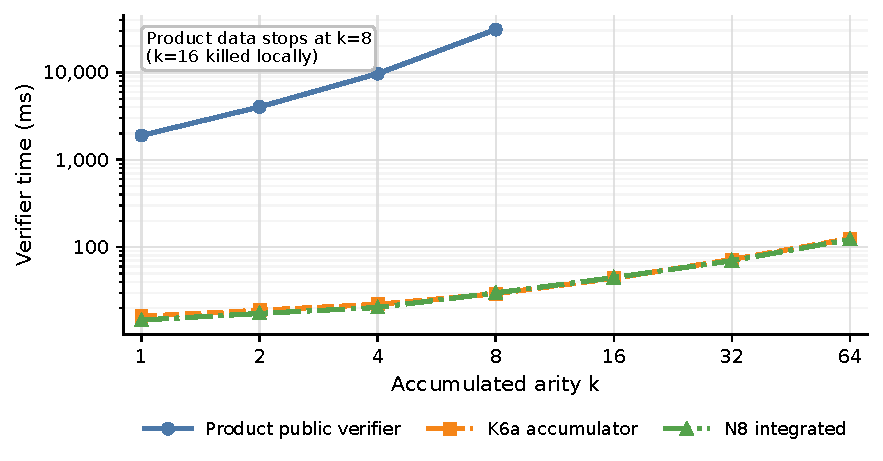
\includegraphics[width=0.85\linewidth]{figures/eval_verify_time.pdf}
\caption{Verifier time versus accumulated arity. K6a and N8 nearly overlap in
this benchmark; both are shown with distinct markers to make clear that they are
separate explicit routes. The product public verifier is the authoritative
baseline and only completed through \(k=8\) locally.}
\label{fig:eval-verify-time}
\end{figure}

\begin{figure}[htbp]
\centering
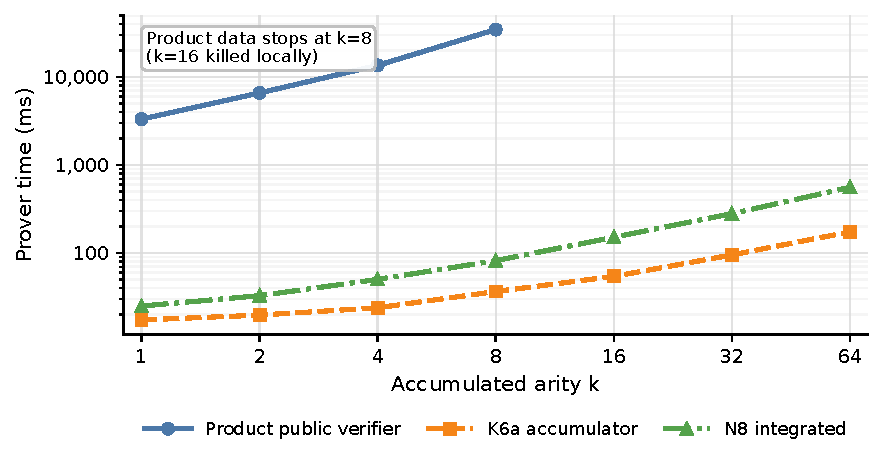
\includegraphics[width=0.85\linewidth]{figures/eval_prove_time.pdf}
\caption{Prover time versus accumulated arity for the product baseline, K6a
accumulator, and N8 integrated route. Product-route rows stop at \(k=8\) because
the local \(k=16\) product benchmark was killed by the operating system.}
\label{fig:eval-prove-time}
\end{figure}

%%%%%%%%%%%%%%%%%%%%%%%%%%%%%%%%%%%%%%%%%%%%%%%%%%%%%%%%%%%%
\subsection{K6a Explicit Accumulator Route}
\label{sec:k6a-explicit-accumulator-route}
%%%%%%%%%%%%%%%%%%%%%%%%%%%%%%%%%%%%%%%%%%%%%%%%%%%%%%%%%%%%

The K6a route replaces the monolithic product public-verifier workload by one
explicit accumulator transition:
\[
  \mathsf{AccVerify}
  \left(
    \Acc_{\mathsf{old}},
    \{\mathsf{Claim}_i\}_{i=1}^k,
    \Acc_{\mathsf{new}},
    \Pi_{\mathsf{acc}}
  \right)=1.
\]
This route is explicit opt-in, NonZK integrity-only, and not the default
\texttt{verify\_public} route. In the benchmarked shape it verifies successfully
for all measured arities, selects the product route, and does not use the
monolithic fallback.

The \emph{Source claims} column in \Cref{tab:k6a-scaling} is the logical source
R1CS residual-claim count, not the number of top-level WHIR proofs. In this
workload each accumulated item contributes 64 such logical source claims, so the
counter is \(64k\); the verifier-side source residual evaluation is compressed
to one batched evaluation in the current K6a profile.

\begin{table}[H]
\centering
\small
\begin{tabular}{rrrrrrr}
\toprule
\(\boldsymbol{k}\) &
\textbf{Prove ms} &
\textbf{Verify ms} &
\textbf{Proof bytes} &
\textbf{Public bytes} &
\textbf{Oracle len.} &
\textbf{Source claims} \\
\midrule
1 & 16.538 & 16.161 & 307,597 & 18,715 & 4,096 & 64 \\
2 & 19.493 & 18.981 & 345,133 & 18,715 & 4,096 & 128 \\
4 & 24.232 & 22.168 & 340,214 & 18,715 & 4,096 & 256 \\
8 & 34.892 & 29.320 & 372,764 & 18,715 & 8,192 & 512 \\
16 & 54.309 & 43.982 & 421,516 & 18,715 & 16,384 & 1,024 \\
32 & 95.278 & 72.256 & 645,435 & 18,715 & 32,768 & 2,048 \\
64 & 174.264 & 125.655 & 682,806 & 18,715 & 65,536 & 4,096 \\
\bottomrule
\end{tabular}
\caption{K6a explicit accumulator scaling from
\texttt{benchmarks/symbt3\_scaling.csv}. The public statement size is flat for
this run, while the logical source-claim counter scales with \(k\).}
\label{tab:k6a-scaling}
\end{table}

\begin{figure}[htbp]
\centering
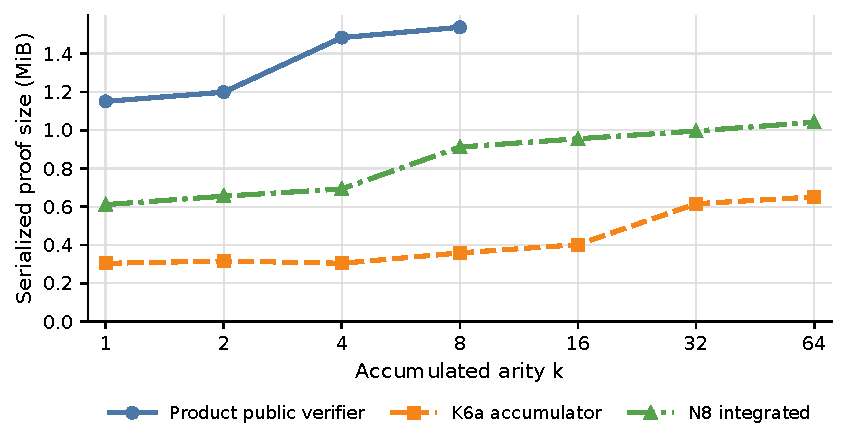
\includegraphics[width=0.85\linewidth]{figures/eval_proof_size.pdf}
\caption{Serialized proof size versus arity. The accumulator routes keep a
single public transition proof shape rather than a list of independent WHIR
proofs.}
\label{fig:eval-proof-size}
\end{figure}

\begin{figure}[htbp]
\centering
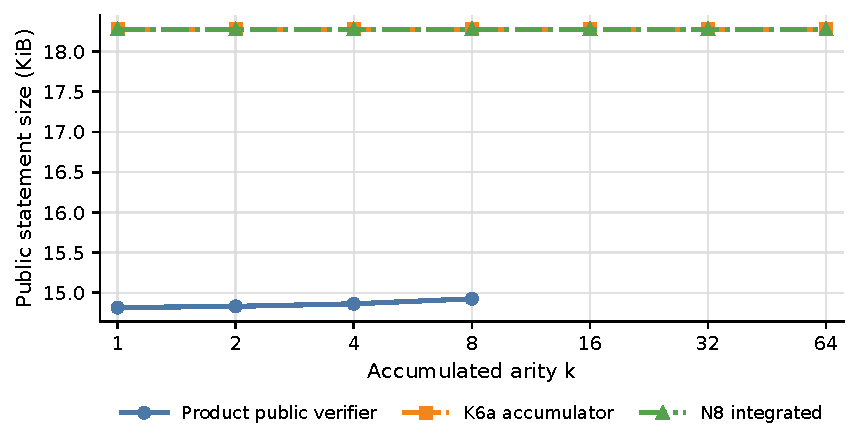
\includegraphics[width=0.85\linewidth]{figures/eval_public_statement_size.pdf}
\caption{Public statement size versus arity. K6a and N8 are flat in the
measured shape because the accumulator boundary is fixed-size for this
workload.}
\label{fig:eval-public-statement-size}
\end{figure}

The generated scaling summary reports log-log slopes of \(0.490\) for
verification time, \(0.569\) for proving time, \(0.199\) for proof bytes, and
\(0.000\) for public statement bytes. The architecture guardrail also remains
stable: one top-level WHIR proof, zero family-columnar subproofs, and one
backend table for every measured \(k\).

%%%%%%%%%%%%%%%%%%%%%%%%%%%%%%%%%%%%%%%%%%%%%%%%%%%%%%%%%%%%
\subsection{N8 Integrated Route and Native Multi-Oracle Evidence}
\label{sec:n8-integrated-evaluation}
%%%%%%%%%%%%%%%%%%%%%%%%%%%%%%%%%%%%%%%%%%%%%%%%%%%%%%%%%%%%

The N8 route is an explicit integrated one-WHIR alternative for same-shape
NonZK accumulation transitions. It is not the default product
\texttt{verify\_public} route, but it is useful evidence for the direction of
the implementation: the public route can be expressed through a more integrated
native-oracle structure rather than only through the K6a wrapper-style path.

\begin{table}[H]
\centering
\small
\begin{tabular}{rrrrrrrr}
\toprule
\(\boldsymbol{k}\) &
\textbf{Status} &
\textbf{Prove ms} &
\textbf{Verify ms} &
\textbf{Proof bytes} &
\textbf{WHIR inst.} &
\textbf{Roots} &
\textbf{Soundness bits} \\
\midrule
1 & OK & 24.979 & 14.670 & 640,702 & 1 & 1 & 124 \\
2 & OK & 32.787 & 17.446 & 686,949 & 1 & 1 & 124 \\
4 & OK & 50.262 & 20.378 & 726,636 & 1 & 1 & 124 \\
8 & OK & 81.866 & 29.977 & 956,339 & 1 & 1 & 124 \\
16 & OK & 151.373 & 44.832 & 1,001,709 & 1 & 1 & 124 \\
32 & OK & 280.310 & 69.956 & 1,044,400 & 1 & 1 & 124 \\
64 & OK & 558.118 & 122.412 & 1,091,966 & 1 & 1 & 124 \\
\bottomrule
\end{tabular}
\caption{N8 integrated explicit route from
\texttt{benchmarks/n8\_integrated\_authority.csv}. All measured rows pass the
N8 authority gate with complete K6a, tuple-RLC, and transition semantics.}
\label{tab:n8-integrated}
\end{table}

\begin{figure}[htbp]
\centering
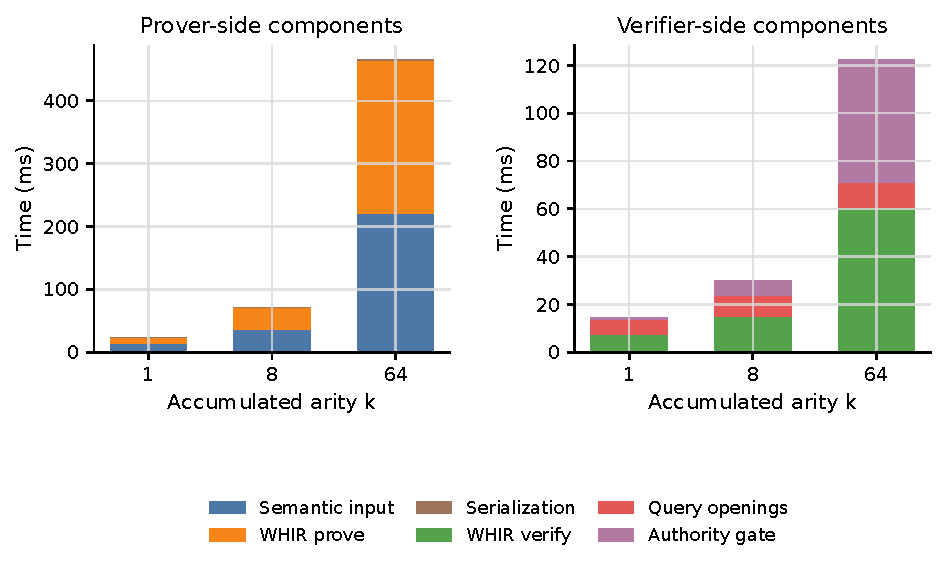
\includegraphics[width=0.85\linewidth]{figures/eval_n8_timer_breakdown.pdf}
\caption{N8 timing breakdown for representative arities. The dominant
components identify the remaining implementation bottlenecks.}
\label{fig:eval-n8-timer-breakdown}
\end{figure}

The native multi-oracle instrumentation is not the main accumulator workload,
but it records the intended tuple-leaf shape. In the refreshed JSONL run over
logical-oracle counts \(1,2,4,8,16,32,64\), every true native tuple-leaf row
passes the shape guard and uses one WHIR instance, one root, one query schedule,
and one transcript. For the \(k_{\mathsf{table}}=8\), 64-logical-oracle row, the
tuple-leaf verifier measurement is \(0.516\) ms against \(30.683\) ms for the
corresponding \(n\)-times-single-oracle baseline.

%%%%%%%%%%%%%%%%%%%%%%%%%%%%%%%%%%%%%%%%%%%%%%%%%%%%%%%%%%%%
\subsection{Bottleneck Analysis}
\label{sec:bottleneck-analysis}
%%%%%%%%%%%%%%%%%%%%%%%%%%%%%%%%%%%%%%%%%%%%%%%%%%%%%%%%%%%%

The current implementation identifies three main bottlenecks.

First, the authoritative product public verifier remains expensive because the
monolithic typed-CP relation is large. This route is still the correct public
baseline: a first unoptimized, monolithic implementation that is expected to
pass for honest public WHIR proofs and fail closed for malformed public data.
The local timings nevertheless show seconds of verifier work even for small
\(k\). The local monolithic run did not reach \(k=16\), which reinforces that
this baseline is not the intended accumulated cost profile.

Second, public binding material is not free. In the K6a route the public
statement is 18,715 bytes for all measured \(k\), slightly larger than the
product public envelope. The main public-byte contributors are folded values,
the accumulator boundary, and relation/output digests. This material is
soundness-critical and should not be removed without an equivalence audit.

Third, the explicit accumulator routes are NonZK integrity-only. K6a is the
current full-workload accumulation path and N8 is the integrated explicit
alternative, but neither should be described as the default product
\texttt{verify\_public} route or as a production zero-knowledge accumulator.

The evaluation should therefore be read as a measurement of current route shape
and public-verifier cost, not as the final performance profile of an optimized
native multi-oracle accumulator. The key result is nevertheless clear: the
explicit accumulator routes check one public transition and avoid the repeated
monolithic public-verifier cost that dominates the baseline.


%%%%%%%%%%%%%%%%%%%%%%%%%%%%%%%%%%%%%%%%%%%%%%%%%%%%%%%%%%%%
\section{Challenges and Limitations}
\label{sec:challenges-limitations}
%%%%%%%%%%%%%%%%%%%%%%%%%%%%%%%%%%%%%%%%%%%%%%%%%%%%%%%%%%%%

The construction and soundness argument above are intentionally conditional.
They identify the interface required for a sound WHIR-backed accumulator, but
they do not by themselves imply that every implementation route realizes this
interface in a production-authoritative way. This section records the main
remaining challenges.

%%%%%%%%%%%%%%%%%%%%%%%%%%%%%%%%%%%%%%%%%%%%%%%%%%%%%%%%%%%%
\subsection{Relation Encoding}
\label{sec:relation-encoding-limitations}
%%%%%%%%%%%%%%%%%%%%%%%%%%%%%%%%%%%%%%%%%%%%%%%%%%%%%%%%%%%%

The most important limitation is relation encoding. The soundness theorem applies
only if the WHIR backend statement faithfully encodes the intended CP folding
relation. In particular, the backend relation must bind the same old accumulator,
new accumulator, claim batch, transcript material, backend parameters, and
folded-output boundary as the public verifier.

This is not merely a formatting requirement. If the WHIR backend proves a
strictly weaker relation, omits part of the CP instance, or proves the folding
transition under different public metadata, then backend soundness applies to the
wrong language. In that case the WHIR proof may be valid while the accumulator
transition is not sound for the intended public statement.

The implemented routes therefore have to be checked against the relation ledger
of Section~\ref{sec:formal-relations}. In particular, the typed SYMBT3/K6a/N8
rows must represent the same proof-validity obligations as the abstract claims
used in the soundness theorem. This is the main mathematical interface between
the implementation and the proof.

%%%%%%%%%%%%%%%%%%%%%%%%%%%%%%%%%%%%%%%%%%%%%%%%%%%%%%%%%%%%
\subsection{Commitment Compatibility}
\label{sec:commitment-compatibility-limitations}
%%%%%%%%%%%%%%%%%%%%%%%%%%%%%%%%%%%%%%%%%%%%%%%%%%%%%%%%%%%%

The construction uses several commitment layers with different purposes. The
lattice/Ajtai-style commitments bind folding data and openings. The
commit-and-prove layer binds the witness material used to certify the folding
transition. The WHIR backend uses oracle commitments, typically represented by
hash or Merkle-style commitments, to make the encoded CP relation succinctly
verifiable.

These layers must not be conflated. A commitment that binds a WHIR oracle does
not automatically bind an Ajtai opening, and an Ajtai commitment does not
automatically bind the public WHIR transcript. Soundness requires that all
commitment layers be tied to the same public statement through explicit digests,
relation identifiers, transcript roots, and accumulator boundaries.

A production implementation should therefore maintain a clear separation between
commitment roles, while ensuring that the final public verifier checks that all
commitment layers refer to the same accumulator transition.

%%%%%%%%%%%%%%%%%%%%%%%%%%%%%%%%%%%%%%%%%%%%%%%%%%%%%%%%%%%%
\subsection{Transcript Binding}
\label{sec:transcript-binding-limitations}
%%%%%%%%%%%%%%%%%%%%%%%%%%%%%%%%%%%%%%%%%%%%%%%%%%%%%%%%%%%%

Transcript binding is another major soundness boundary. The folding challenges,
WHIR backend challenges, and public verifier digests must be derived from the
same public statement material. A prover should not be able to derive challenges
from one transcript and then present the resulting proof under a different public
boundary.

In this report, the transcript-binding requirement appears in several places:
the WHIR proof-validity claims, the folding challenge derivation, the CP public
instance, and the backend WHIR statement. The implementation must ensure that
all these views agree. The relevant public material includes relation metadata,
public inputs, transcript roots, challenge digests, folded-output boundaries,
and accumulator identifiers.

The fail-closed verifier boundary is essential here. If the verifier cannot
recompute or validate the transcript binding from public data, it should reject
rather than replaying prover-side material or using a debug helper.

%%%%%%%%%%%%%%%%%%%%%%%%%%%%%%%%%%%%%%%%%%%%%%%%%%%%%%%%%%%%
\subsection{Prototype Boundaries}
\label{sec:prototype-boundaries}
%%%%%%%%%%%%%%%%%%%%%%%%%%%%%%%%%%%%%%%%%%%%%%%%%%%%%%%%%%%%

The report distinguishes between the semantic accumulator and the implemented
routes. The abstract notation uses a batch of WHIR proof-validity claims
\[
  \{\mathsf{Claim}_i\}_{i=1}^k,
\]
but the concrete single-oracle and multi-oracle routes consume typed
accumulation batches and route-specific public instances. They should therefore
be understood as implementations of the semantic interface, not as unrestricted
generic accumulators for arbitrary WHIR proof objects.

This distinction matters for evaluation and for soundness claims. The
single-oracle route is the current explicit full-workload accumulation path. The
multi-oracle route is an implemented opt-in alternative, but it is not the
default public verifier and should not be presented as production-reviewed. Both
routes are NonZK integrity-only in the current report.

Thus the implementation should be viewed as a soundness-guided prototype of
WHIR-backed accumulation, not as a complete production implementation of a full
zero-knowledge Symphony-style SNARK.

%%%%%%%%%%%%%%%%%%%%%%%%%%%%%%%%%%%%%%%%%%%%%%%%%%%%%%%%%%%%
\subsection{Remaining Gaps}
\label{sec:remaining-gaps}
%%%%%%%%%%%%%%%%%%%%%%%%%%%%%%%%%%%%%%%%%%%%%%%%%%%%%%%%%%%%

The main remaining gaps are the following.

First, the typed CP relation remains large. The default public verifier preserves
the public boundary, but its cost is still dominated by the monolithic typed CP
relation. This motivates the native and multi-oracle direction.

Second, the relation encoding must be audited carefully. The strongest version
of the construction requires the backend WHIR statement to encode exactly the CP
folding relation. Any mismatch between typed implementation rows and the
abstract relation definitions weakens the soundness theorem.

Third, the implementation is not zero-knowledge. The current accumulation routes
are described as NonZK integrity-only routes. Adding zero-knowledge would require
additional masking/blinding arguments and a separate analysis.

\paragraph{Zero-knowledge.}
The current routes are NonZK integrity-only. Adding zero-knowledge is not a
matter of simply hiding the final accumulator. The prover would need to mask or
blind the folding witness, commitment openings, and auxiliary CP witness data,
and the backend WHIR statement would need to prove the masked CP relation while
binding the masking commitments into the same public transcript.

The performance overhead depends on the chosen zero-knowledge compiler. At a
minimum, one should expect additional committed columns or rows for masks,
additional constraints checking consistency between masked and unmasked
quantities, and additional transcript material binding the masking commitments.
Because the evaluation already identifies the typed CP relation as a dominant
cost, any ZK layer that enlarges this relation may have a meaningful prover-time
impact. Quantifying that overhead requires choosing a concrete ZK transformation
for the CP relation and is left as future work.

Fourth, the current report proves a one-step conditional composition theorem.
For long accumulation chains, the error terms and accumulator invariants must be
tracked across multiple steps. The simple bound in Section~\ref{sec:error-composition}
scales with the number of accumulation steps unless a tighter analysis is used.

Finally, a production-authoritative route would need a complete public-verifier
audit: no witness-side replay, no debug-only fallback, no non-authoritative typed
helper, and explicit binding of all public statement components.

%%%%%%%%%%%%%%%%%%%%%%%%%%%%%%%%%%%%%%%%%%%%%%%%%%%%%%%%%%%%
\section{Related Work}
\label{sec:related-work}
%%%%%%%%%%%%%%%%%%%%%%%%%%%%%%%%%%%%%%%%%%%%%%%%%%%%%%%%%%%%

This report sits at the intersection of four lines of work: WHIR-style
hash-based proof backends, lattice-based folding, commit-and-prove SNARKs, and
accumulation schemes. We discuss each in turn and explain how the present
construction differs from prior work.

%%%%%%%%%%%%%%%%%%%%%%%%%%%%%%%%%%%%%%%%%%%%%%%%%%%%%%%%%%%%
\subsection{WHIR and Reed--Solomon Proximity Testing}
%%%%%%%%%%%%%%%%%%%%%%%%%%%%%%%%%%%%%%%%%%%%%%%%%%%%%%%%%%%%

WHIR~\cite{WHIR} is an interactive oracle proof of proximity for constrained
Reed--Solomon codes with small query complexity and very fast verification. It
can serve as a backend for polynomial-IOP style proof systems, replacing or
improving on earlier Reed--Solomon proximity-testing components such as
FRI~\cite{FRI}, STIR~\cite{STIR}, and BaseFold-style
folding~\cite{BaseFold}. Its verifier efficiency makes it attractive as a public
proof backend.

The present report uses WHIR in two different roles. First, the input objects
being accumulated are WHIR-backed proof-validity claims. Second, WHIR is used
again as the backend proof system for the commit-and-prove relation that
certifies the folding transition. This differs from using WHIR only as a
standalone proof system: the central question here is whether WHIR verification
claims can themselves be accumulated without losing the public soundness
boundary.

%%%%%%%%%%%%%%%%%%%%%%%%%%%%%%%%%%%%%%%%%%%%%%%%%%%%%%%%%%%%
\subsection{Symphony and Lattice-Based Folding}
%%%%%%%%%%%%%%%%%%%%%%%%%%%%%%%%%%%%%%%%%%%%%%%%%%%%%%%%%%%%

Symphony~\cite{Symphony} proposes a lattice-based high-arity folding framework for
building scalable SNARKs in the random oracle model. Its key architectural idea
is to use high-arity folding together with a commit-and-prove compiler, while
avoiding the need to place Fiat--Shamir hash computations inside the proved
statements. This makes Symphony a natural starting point for studying
memory-efficient and potentially post-quantum accumulation architectures.

Our construction follows the Symphony-style viewpoint that a folding transition
should be certified by a CP relation, rather than by exposing prover-side
folding witnesses to the public verifier. However, the goal here is narrower:
we do not claim to implement a full production Symphony SNARK. Instead, we study
the specific composition problem that arises when WHIR-backed proof-validity
claims are folded through a Symphony-style accumulator and the resulting CP
relation is itself proved with WHIR.

%%%%%%%%%%%%%%%%%%%%%%%%%%%%%%%%%%%%%%%%%%%%%%%%%%%%%%%%%%%%
\subsection{Commit-and-Prove SNARKs}
%%%%%%%%%%%%%%%%%%%%%%%%%%%%%%%%%%%%%%%%%%%%%%%%%%%%%%%%%%%%

Commit-and-prove SNARKs allow a prover to prove a relation while also proving
consistency with previously committed data. In the present construction, the CP
layer is the bridge between the semantic folding relation and the public backend
proof. It certifies that the prover-side folding witness, openings, and auxiliary
data are consistent with the public accumulator transition, while keeping those
objects outside the public verifier boundary.

The CP layer is also where the main faithfulness requirement arises. The backend
proof system is sound only for the relation it actually encodes. Therefore, the
WHIR backend statement must encode exactly the CP folding relation for the same
public instance: the same old accumulator, new accumulator, claim batch,
transcript-binding material, and folded-output boundary. This faithfulness
condition is what prevents the backend from proving a weaker relation than the
one required by the accumulator.

%%%%%%%%%%%%%%%%%%%%%%%%%%%%%%%%%%%%%%%%%%%%%%%%%%%%%%%%%%%%
\subsection{Accumulation and Folding Schemes}
%%%%%%%%%%%%%%%%%%%%%%%%%%%%%%%%%%%%%%%%%%%%%%%%%%%%%%%%%%%%

Accumulation and folding schemes are widely used to reduce the cost of verifying
many related proof obligations. Instead of recursively verifying every proof
inside another proof system, an accumulator maintains a smaller state that
represents the validity of many prior claims. This idea underlies many modern
incrementally verifiable computation and proof-carrying-data systems.

Recent work explores different accumulation tradeoffs. WARP gives a
hash-based accumulation scheme with linear prover time and logarithmic verifier
time~\cite{WARP}. Quasar studies sublinear accumulation for multiple
instances, aiming to reduce the verifier work associated with accumulating many
predicate instances~\cite{Quasar}. These works are close in spirit to the
present report because they also target the repeated-verification bottleneck.

The difference is the object being accumulated. This report focuses specifically
on WHIR-backed proof-validity claims and on their composition with a
Symphony-style lattice-folding and CP-SNARK architecture. The main question is
not only whether accumulation can reduce verifier work, but whether the
verification relation induced by WHIR proofs can be folded and re-proved with
WHIR while preserving the public verifier boundary.

%%%%%%%%%%%%%%%%%%%%%%%%%%%%%%%%%%%%%%%%%%%%%%%%%%%%%%%%%%%%
\subsection{Transparent SNARKs and Spartan}
%%%%%%%%%%%%%%%%%%%%%%%%%%%%%%%%%%%%%%%%%%%%%%%%%%%%%%%%%%%%

Spartan~\cite{Spartan} is an important transparent SNARK construction for R1CS
that combines sumcheck-style protocols, polynomial commitments, and
preprocessing ideas to obtain succinct verification without a trusted setup.
Spartan is relevant background for this report because it illustrates a
recurring theme in modern proof systems: arithmetize the computation, bind the
public relation carefully, and use polynomial-commitment machinery to obtain
succinct verification.

The present work is not a Spartan-style construction. It does not build a new
R1CS SNARK from scratch. Instead, it assumes a WHIR-backed proving stack and
studies whether the resulting proof-validity claims can be accumulated through
lattice-based folding. Spartan is therefore best viewed as part of the broader
context of transparent succinct proof systems, rather than as a direct component
of the construction.

%%%%%%%%%%%%%%%%%%%%%%%%%%%%%%%%%%%%%%%%%%%%%%%%%%%%%%%%%%%%
\subsection{Positioning of This Work}
%%%%%%%%%%%%%%%%%%%%%%%%%%%%%%%%%%%%%%%%%%%%%%%%%%%%%%%%%%%%

The contribution of this report is not a new low-degree test, a new polynomial
commitment scheme, or a complete new SNARK. Its contribution is a soundness- and
implementation-oriented study of a particular composition:
\[
  \begin{aligned}
  \text{WHIR proof-validity claims}
  &\longrightarrow \text{lattice-based folding}\\
  &\longrightarrow \text{commit-and-prove relation}\\
  &\longrightarrow \text{WHIR backend proof}.
  \end{aligned}
\]
The main novelty is the interface question. WHIR and Symphony each provide
useful components, but their composition is not automatic. The CP relation must
prove the correct folding transition, the WHIR backend must faithfully encode
that CP relation, and the public verifier must remain fail-closed and
authoritative. This report makes those obligations explicit and evaluates the
current implementation routes against them.

 %%%%%%%%%%%%%%%%%%%%%%%%%%%%%%%%%%%%%%%%%%%%%%%%%%%%%%%%%%%%
\section{Future Work}
\label{sec:future-work}
%%%%%%%%%%%%%%%%%%%%%%%%%%%%%%%%%%%%%%%%%%%%%%%%%%%%%%%%%%%%

The implementation and analysis in this report suggest several directions for
future work.

\paragraph{Faithfulness proof for typed rows.}
The soundness theorem in this report assumes that the typed SYMBT3/K6a/N8 rows
faithfully encode the abstract CP folding relation. Section~\ref{sec:row-level-faithfulness-obligations}
reduces this to six row-level obligations: claim representation, shape
consistency, challenge binding, opening consistency, algebraic folding
consistency, and output consistency. A natural next step is to prove these
obligations directly for the implemented rows. Such a proof should proceed
row family by row family, showing that every public binding condition in
\(\Rcp\) is represented in the backend WHIR statement. This would close the
main gap between the abstract soundness theorem and the concrete implementation.

\paragraph{Quasar-style partial evaluation.}
Quasar is an especially interesting exploratory direction for this project.
The current accumulator routes still carry a large typed CP relation, and the
evaluation shows that this relation remains a dominant cost. Quasar-style
multi-instance accumulation suggests a different way to reduce verifier work:
replace some random-linear-combination style verifier operations with partial
evaluation techniques that are sublinear in the number of accumulated instances.
An interesting next step would be to study whether the WHIR-backed CP relation
can be reorganized so that the accumulator verifier checks a smaller partially
evaluated object rather than a monolithic folded relation. This would not replace
the soundness interface developed in this report, but it could provide a more
efficient realization of the same public-boundary requirements.

\paragraph{Zero-knowledge.}
The current routes are NonZK integrity-only. Adding zero-knowledge would require
masking or blinding the relevant witness material, proving that the resulting
distribution hides the private folding data, and checking that the WHIR backend
and transcript-binding logic remain compatible with the zero-knowledge layer.
This would also require revisiting the CP relation, since the current report
focuses on public soundness and accumulator integrity rather than witness
privacy.

\paragraph{Long-chain accumulation.}
The current soundness theorem is a one-step theorem. Section~\ref{sec:error-composition}
explains the conservative union-bound extension to \(T\) steps and sketches how
a sharper chain-level analysis might be obtained. A full treatment should define
a chain invariant \(\mathsf{ValidAcc}(\Acc_t)\), prove that each accepted
transition preserves it, and analyze the entire random-oracle, commitment, and
folding experiment globally rather than as \(T\) independent one-step
experiments.

\paragraph{Broader comparisons.}
The evaluation in this report compares the product public verifier, the K6a
explicit accumulator route, and the N8 integrated route. A broader comparison
would benchmark the same workloads against other accumulation strategies,
including WARP-style hash-based accumulation and Quasar-style multi-instance
accumulation. Such a comparison would clarify whether the main cost in this
project comes from WHIR backend proving, typed CP relation size, transcript
binding, or the specific lattice-folding interface.

%%%%%%%%%%%%%%%%%%%%%%%%%%%%%%%%%%%%%%%%%%%%%%%%%%%%%%%%%%%%
\section{Conclusion}
\label{sec:conclusion}
%%%%%%%%%%%%%%%%%%%%%%%%%%%%%%%%%%%%%%%%%%%%%%%%%%%%%%%%%%%%

This report studied whether WHIR proof-validity claims can be accumulated
through Symphony-style lattice-based folding while preserving a public,
fail-closed verifier boundary. The central object is the WHIR verification
claim, including the public transcript and folded-output data that make it
meaningful.

We formalized this composition as a chain of relations: WHIR verification claims
are absorbed by a folding relation, the folding transition is certified by a
commit-and-prove relation, and that CP relation is proved using WHIR as the
backend. We proved completeness and gave a conditional soundness theorem under
backend soundness, folding soundness, commitment binding, transcript binding,
typed-batch faithfulness, and faithful encoding of the CP relation into WHIR.

The implementation results show that the public-verifier boundary can be
preserved in explicit accumulation routes. In the measured workloads, the K6a
route avoids the repeated monolithic public-verifier cost of the product
baseline, while N8 demonstrates an integrated one-WHIR route with stable
authority metadata across arities. At the same time, the evaluation confirms
that the current system is still a prototype: the typed CP relation, transcript
binding, and relation encoding remain the main bottlenecks toward a
production-authoritative WHIR-backed accumulator.
%%%%%%%%%%%%%%%%%%%%%%%%%%%%%%%%%%%%%%%%%%%%%%%%%%%%%%%%%%%%

%%%%%%%%%%%%%%%%%%%%%%%%%%%%%%%%%%%%%%%%%%%%%%%%%%%%%%%%%%%
%%%%%%%%%%%%%%%%%%%%%%%%%%%%%%%%%%%%%%%%%%%%%%%%%%%%%%%%%%%%
\bibliographystyle{alpha}
\bibliography{references}

%%%%%%%%%%%%%%%%%%%%%%%%%%%%%%%%%%%%%%%%%%%%%%%%%%%%%%%%%%%%
\end{document}
